\section{State Estimation of 1D motion using Kalman Filters}
\subsection{Motion and Observation models}\label{sec:kinematics_train}
\begin{enumerate}
\item 
We run the Kalman update after every $\Delta t$ time-step. The state $X_t \in \re^2$ denotes
\begin{align*}
X_t = \begin{bmatrix} x_t \\ \dot{x}_t \end{bmatrix}\\
\end{align*}
\item The initial belief $X_0 \sim \normal(0, 10^{-4} I_2)$. $u_t$ is a scalar. The motion model is
\begin{align*}
X_{t + 1} &= A_t X_{t} + B_t u_t + \epsilon_t\\
\text{where }
A_t &= \begin{bmatrix} 
1 & \Delta t \\ 
0 & 1 
\end{bmatrix}
\text{, }
B_t = \begin{bmatrix} 
\frac{1}{2} \Delta t^2 \\ 
\Delta t 
\end{bmatrix}
\text{, }
\epsilon_t \sim \normal(0, R_t)\\
\text{where }
R_t &= \begin{bmatrix} 
\sigma_x^2 & 0 \\ 
0 & \sigma_{\dot{x}}^2 
\end{bmatrix}
\end{align*}

\item The observations $Z_t \in \re$ are the noisy value of time taken for sound wave to start from $x = 0$, hit the train and come back. The observation model is
\begin{align*}
Z_t &= C_t X_t + \delta_t\\
\text{where } 
C_t &= \begin{bmatrix} 
\frac{2}{v_{sound}} & 0
\end{bmatrix}
\text{, }
\delta_t \sim \normal(0, \sigma_s^2)
\end{align*}
\end{enumerate}
\begin{figure}[H]
    \centering
    \begin{minipage}{0.49\linewidth}
        \centering
        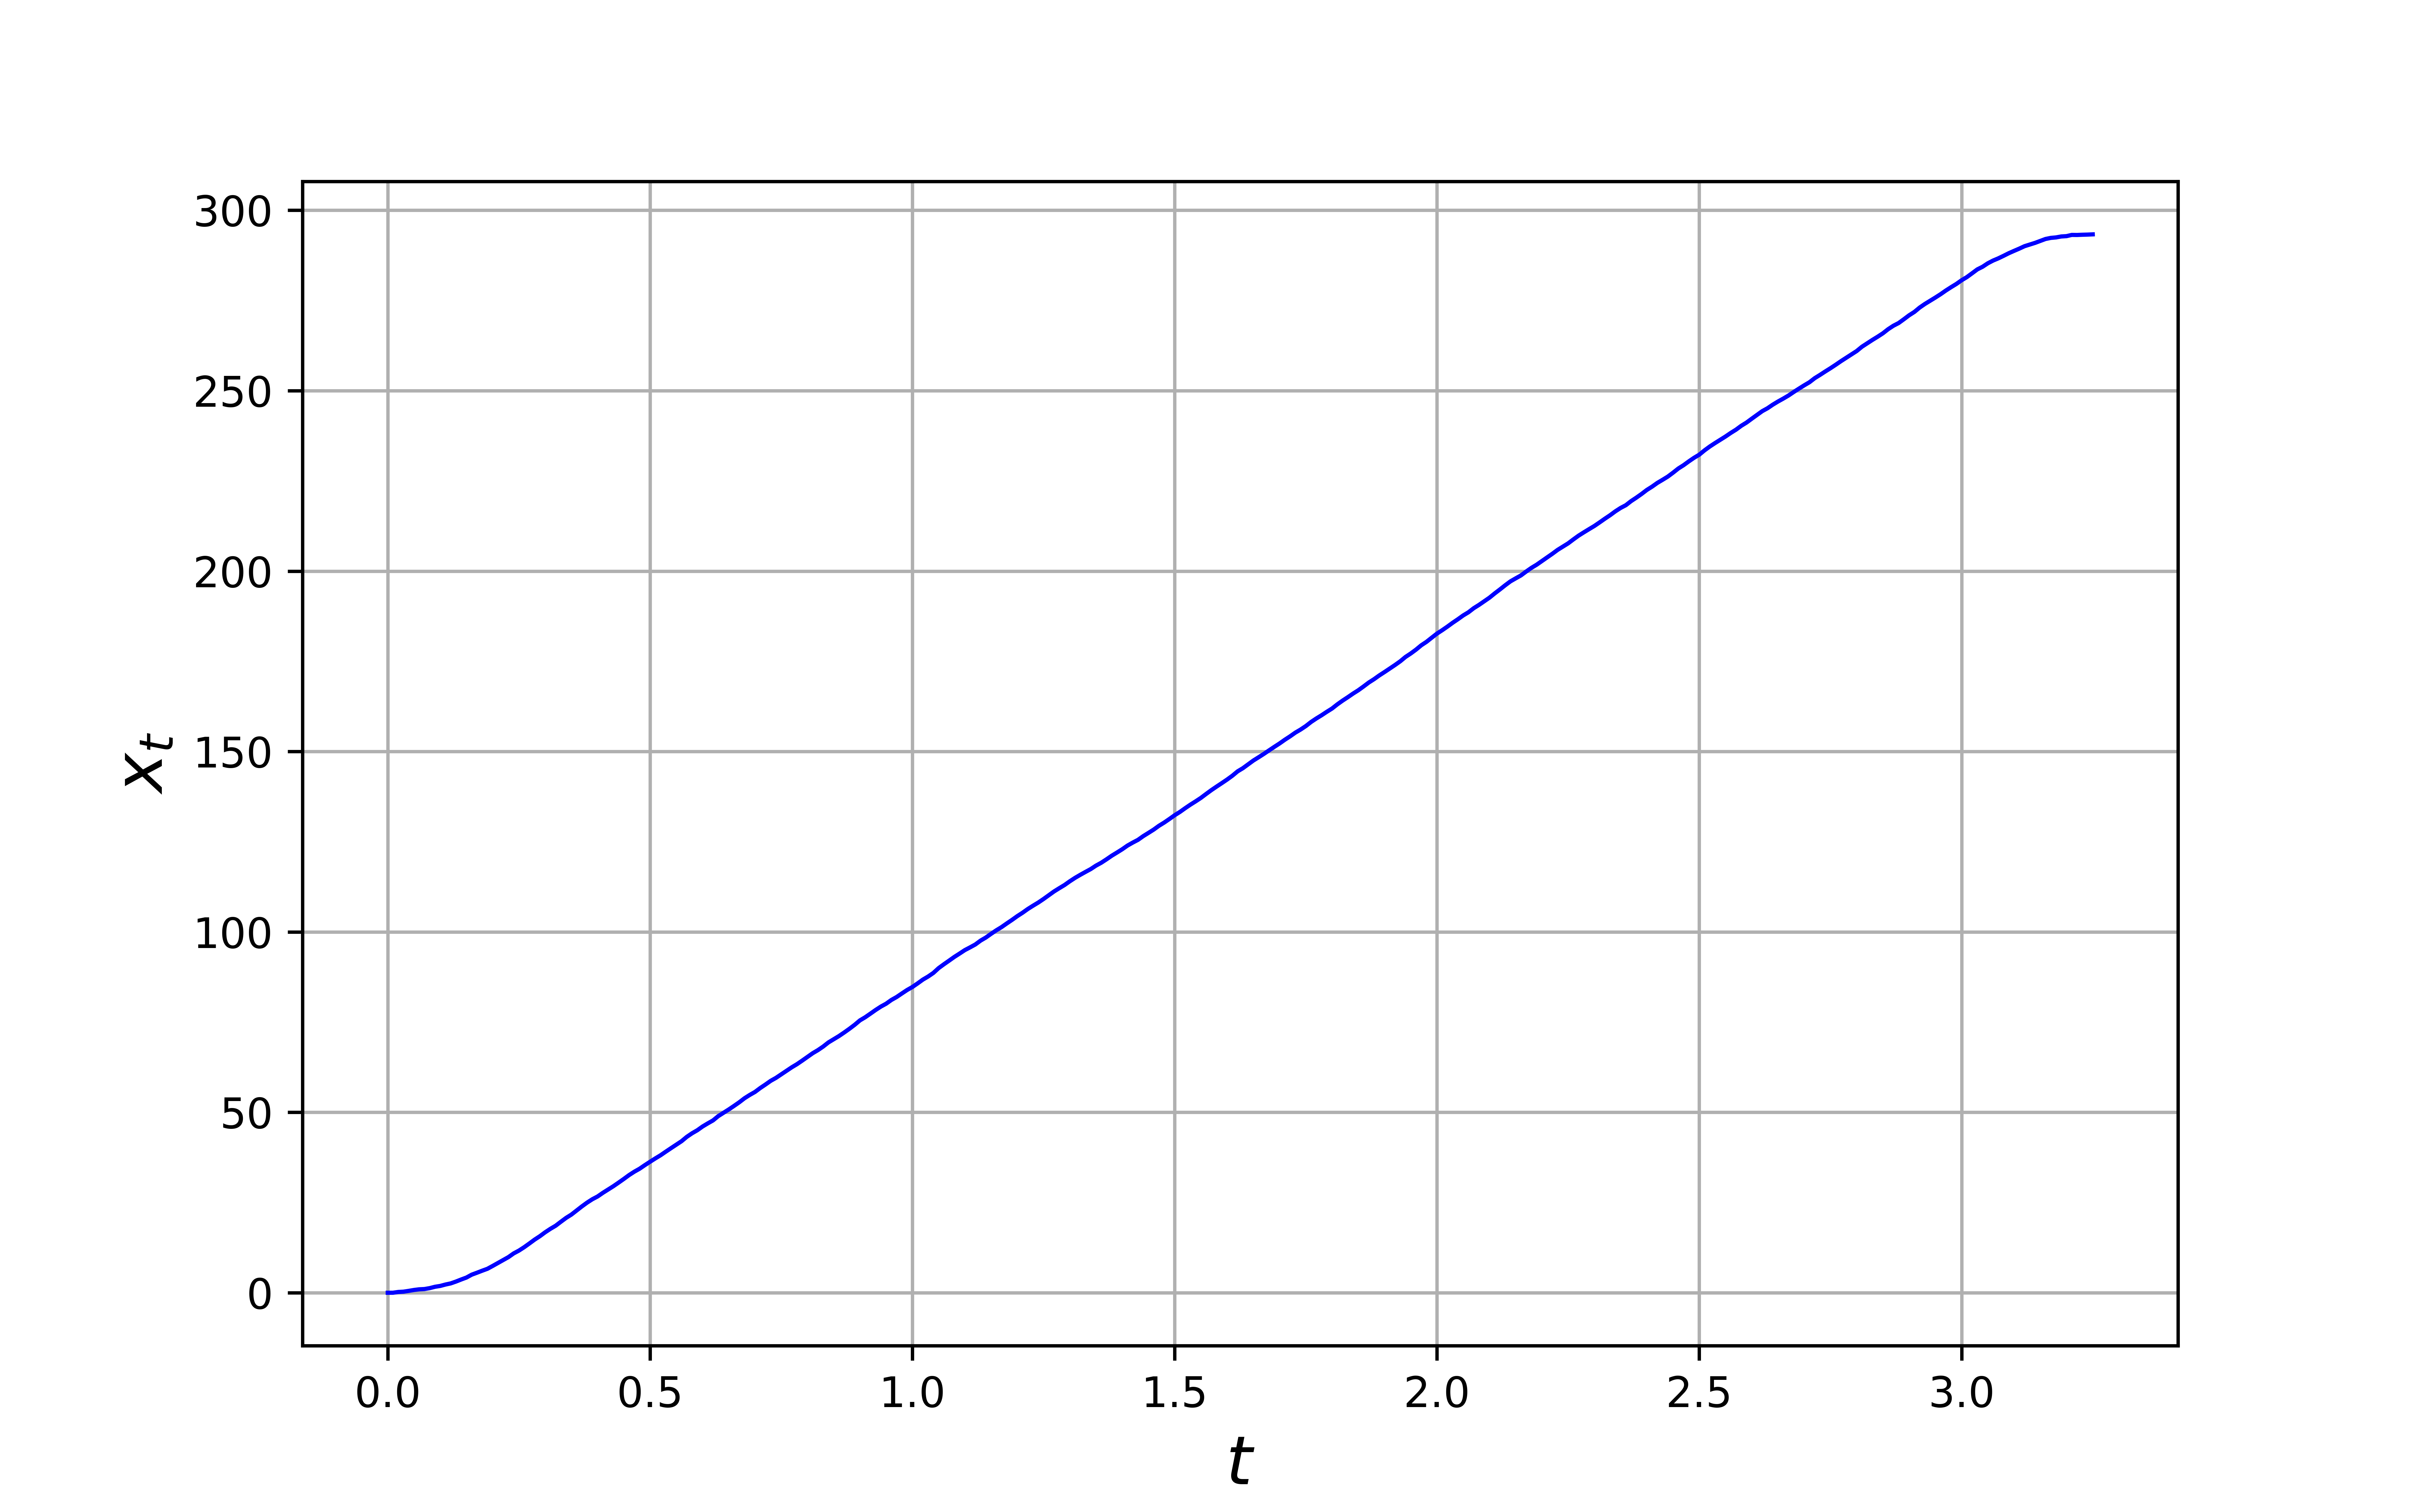
\includegraphics[width=\linewidth]{plots/part1-a.1.png}
        \caption{Ground truth $x_t$ vs $t$}
    \end{minipage}
    \hfill
    \begin{minipage}{0.49\linewidth}
        \centering
        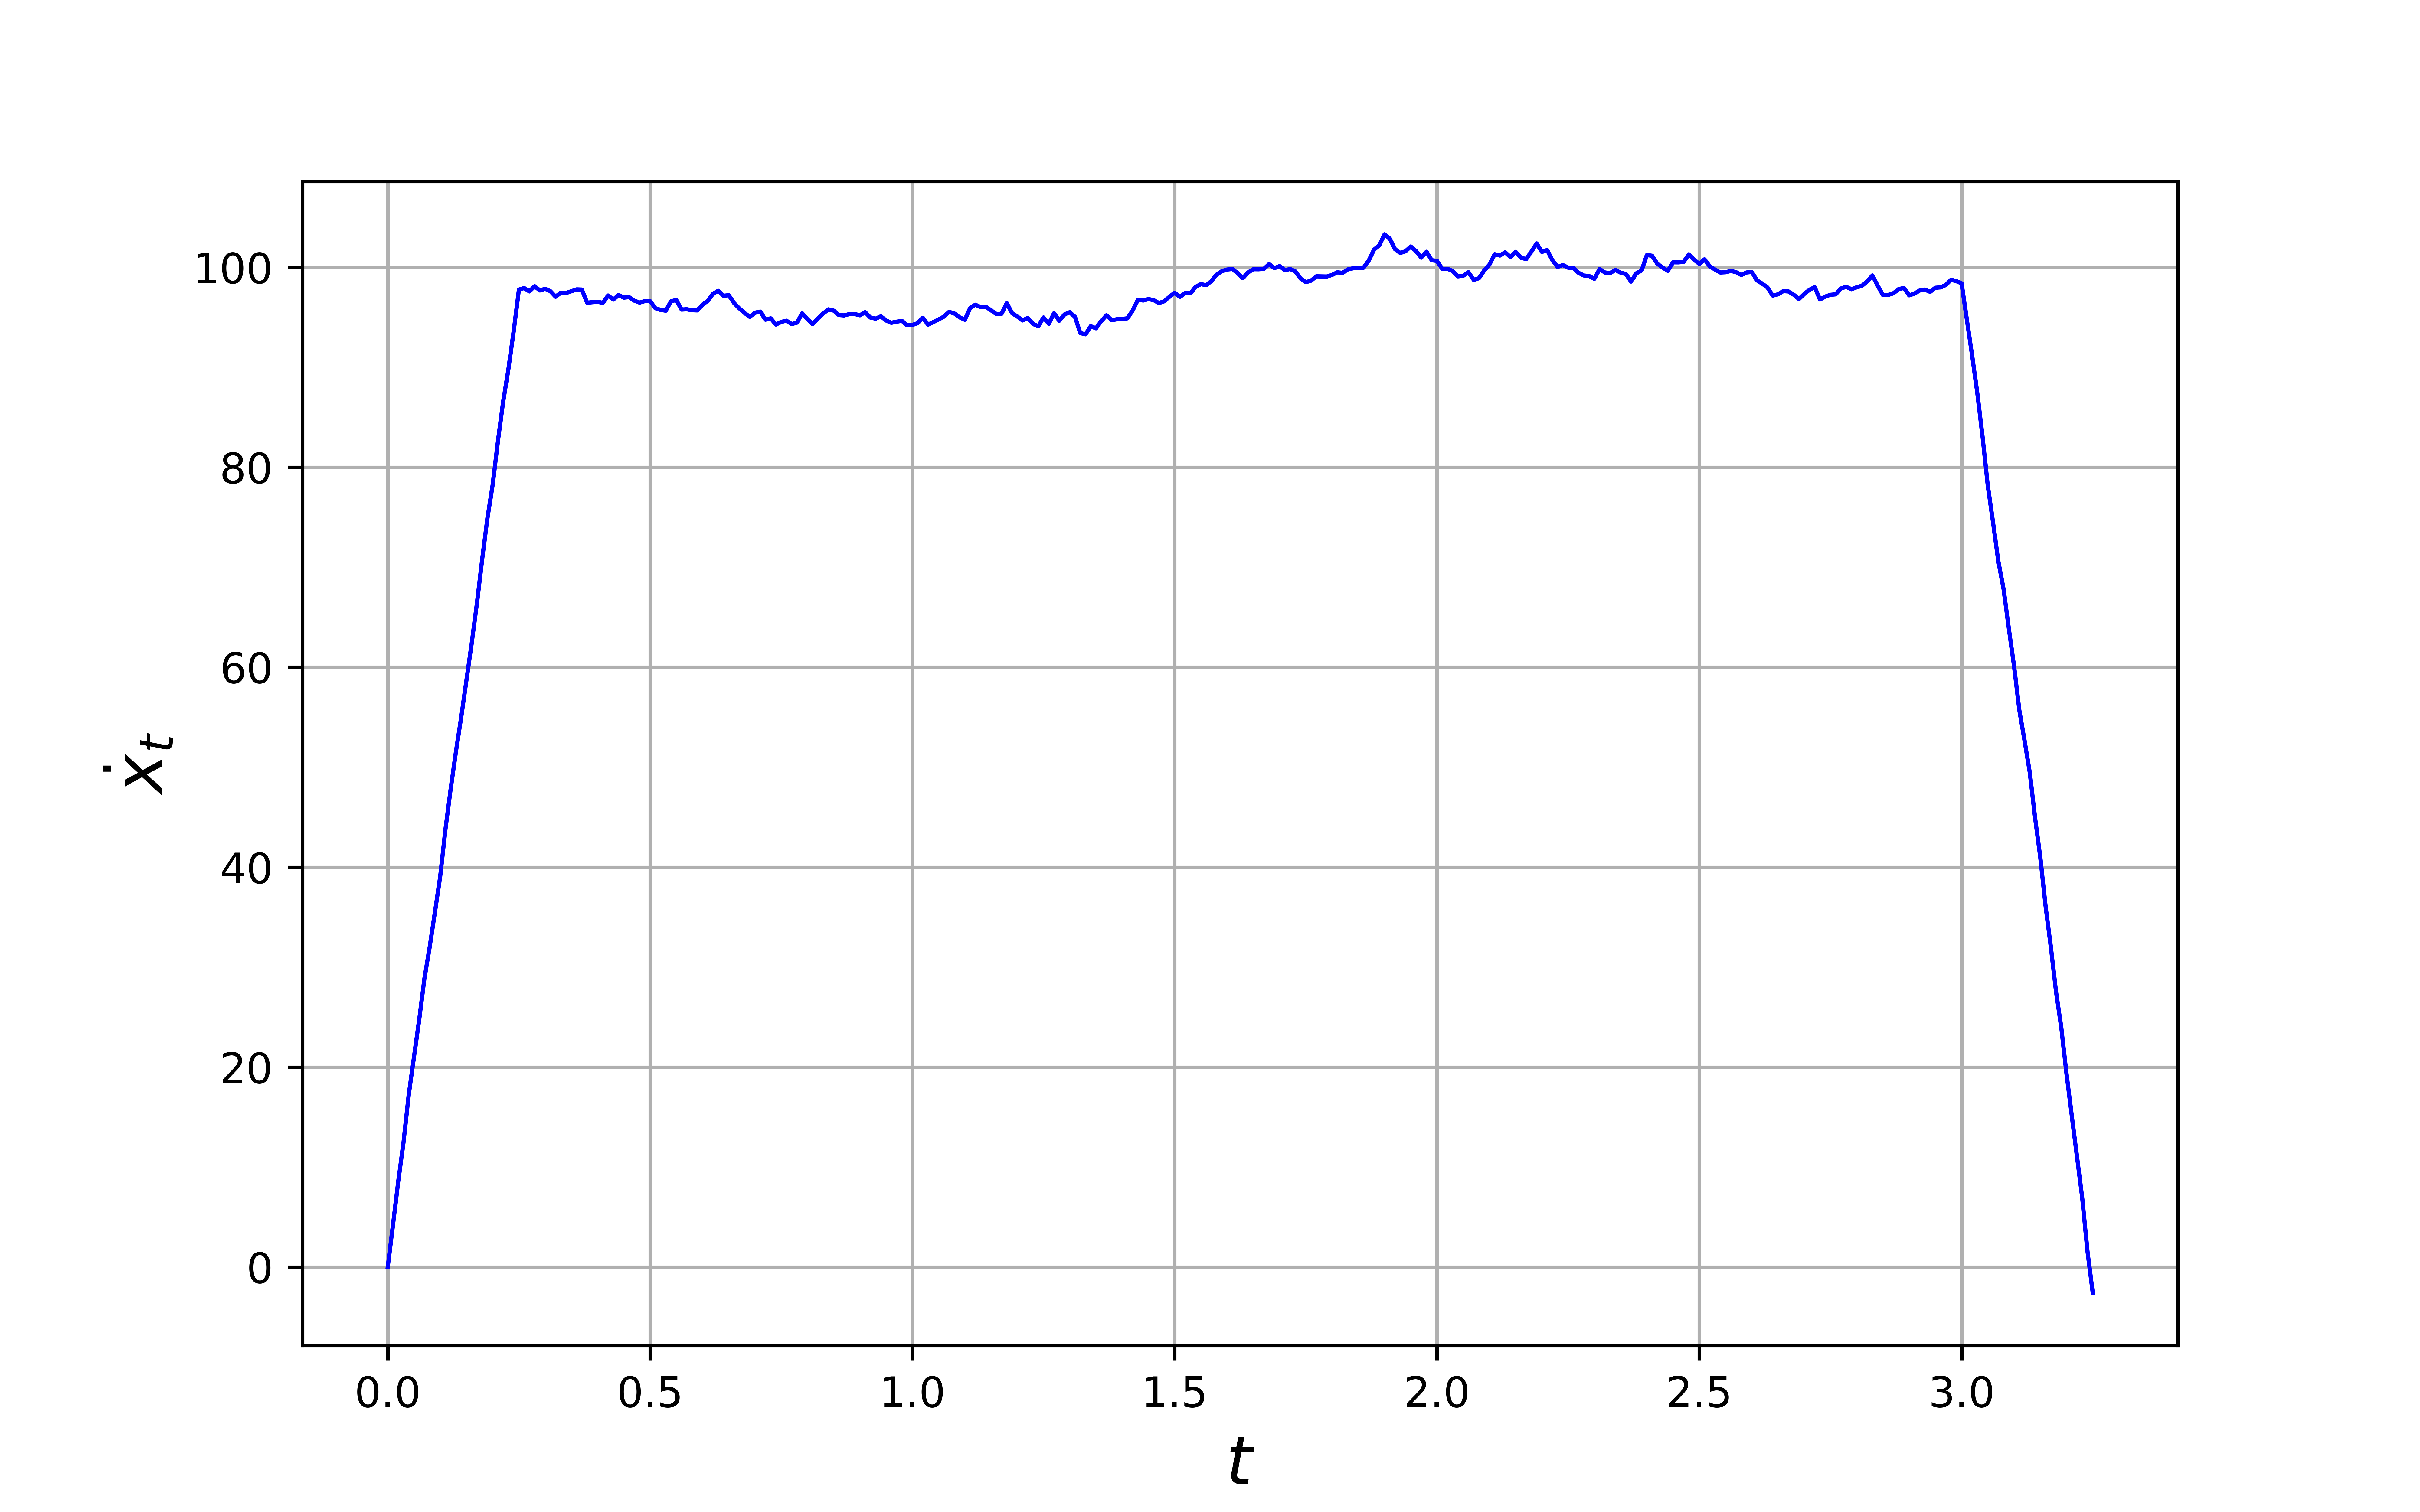
\includegraphics[width=\linewidth]{plots/part1-a.2.png}
        \caption{Ground truth $\dot{x}_t$ vs $t$}
    \end{minipage}
\end{figure}

\begin{figure}[H]
    \centering
    \begin{minipage}{0.49\linewidth}
        \centering
        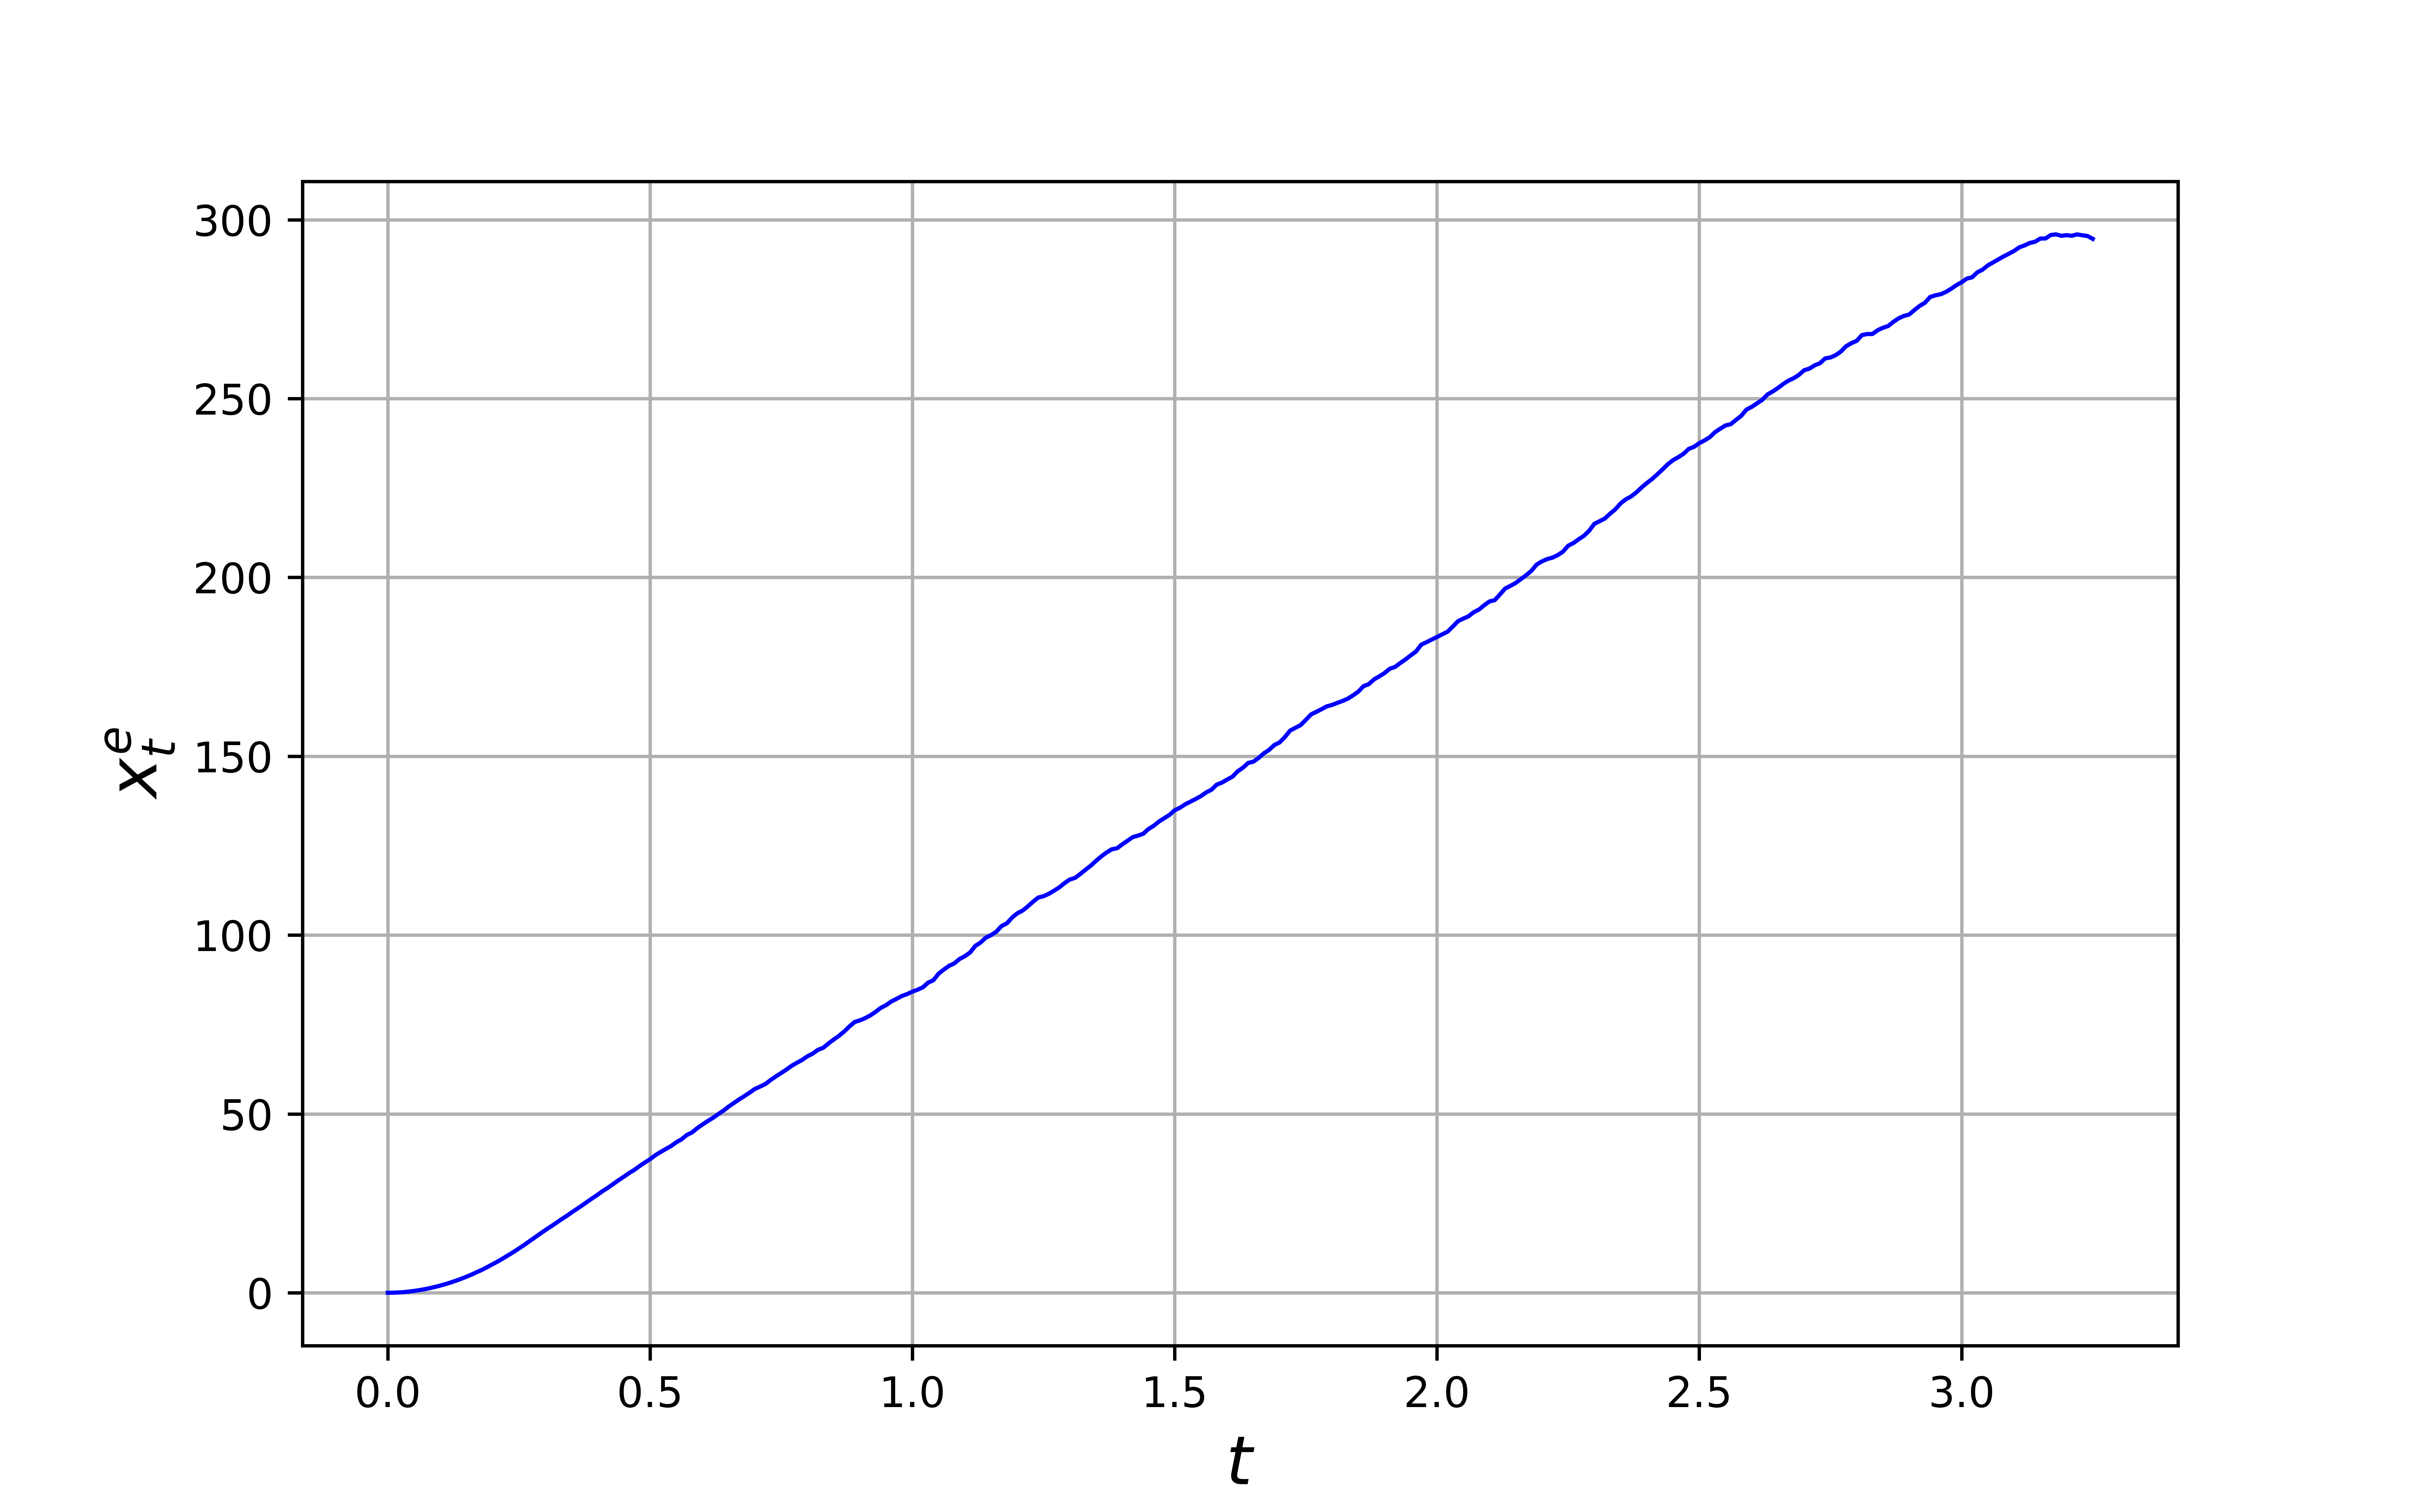
\includegraphics[width=\linewidth]{plots/part1-b.1.png}
        \caption{Estimation $x^e_t$ vs $t$}
    \end{minipage}
    \hfill
    \begin{minipage}{0.49\linewidth}
        \centering
        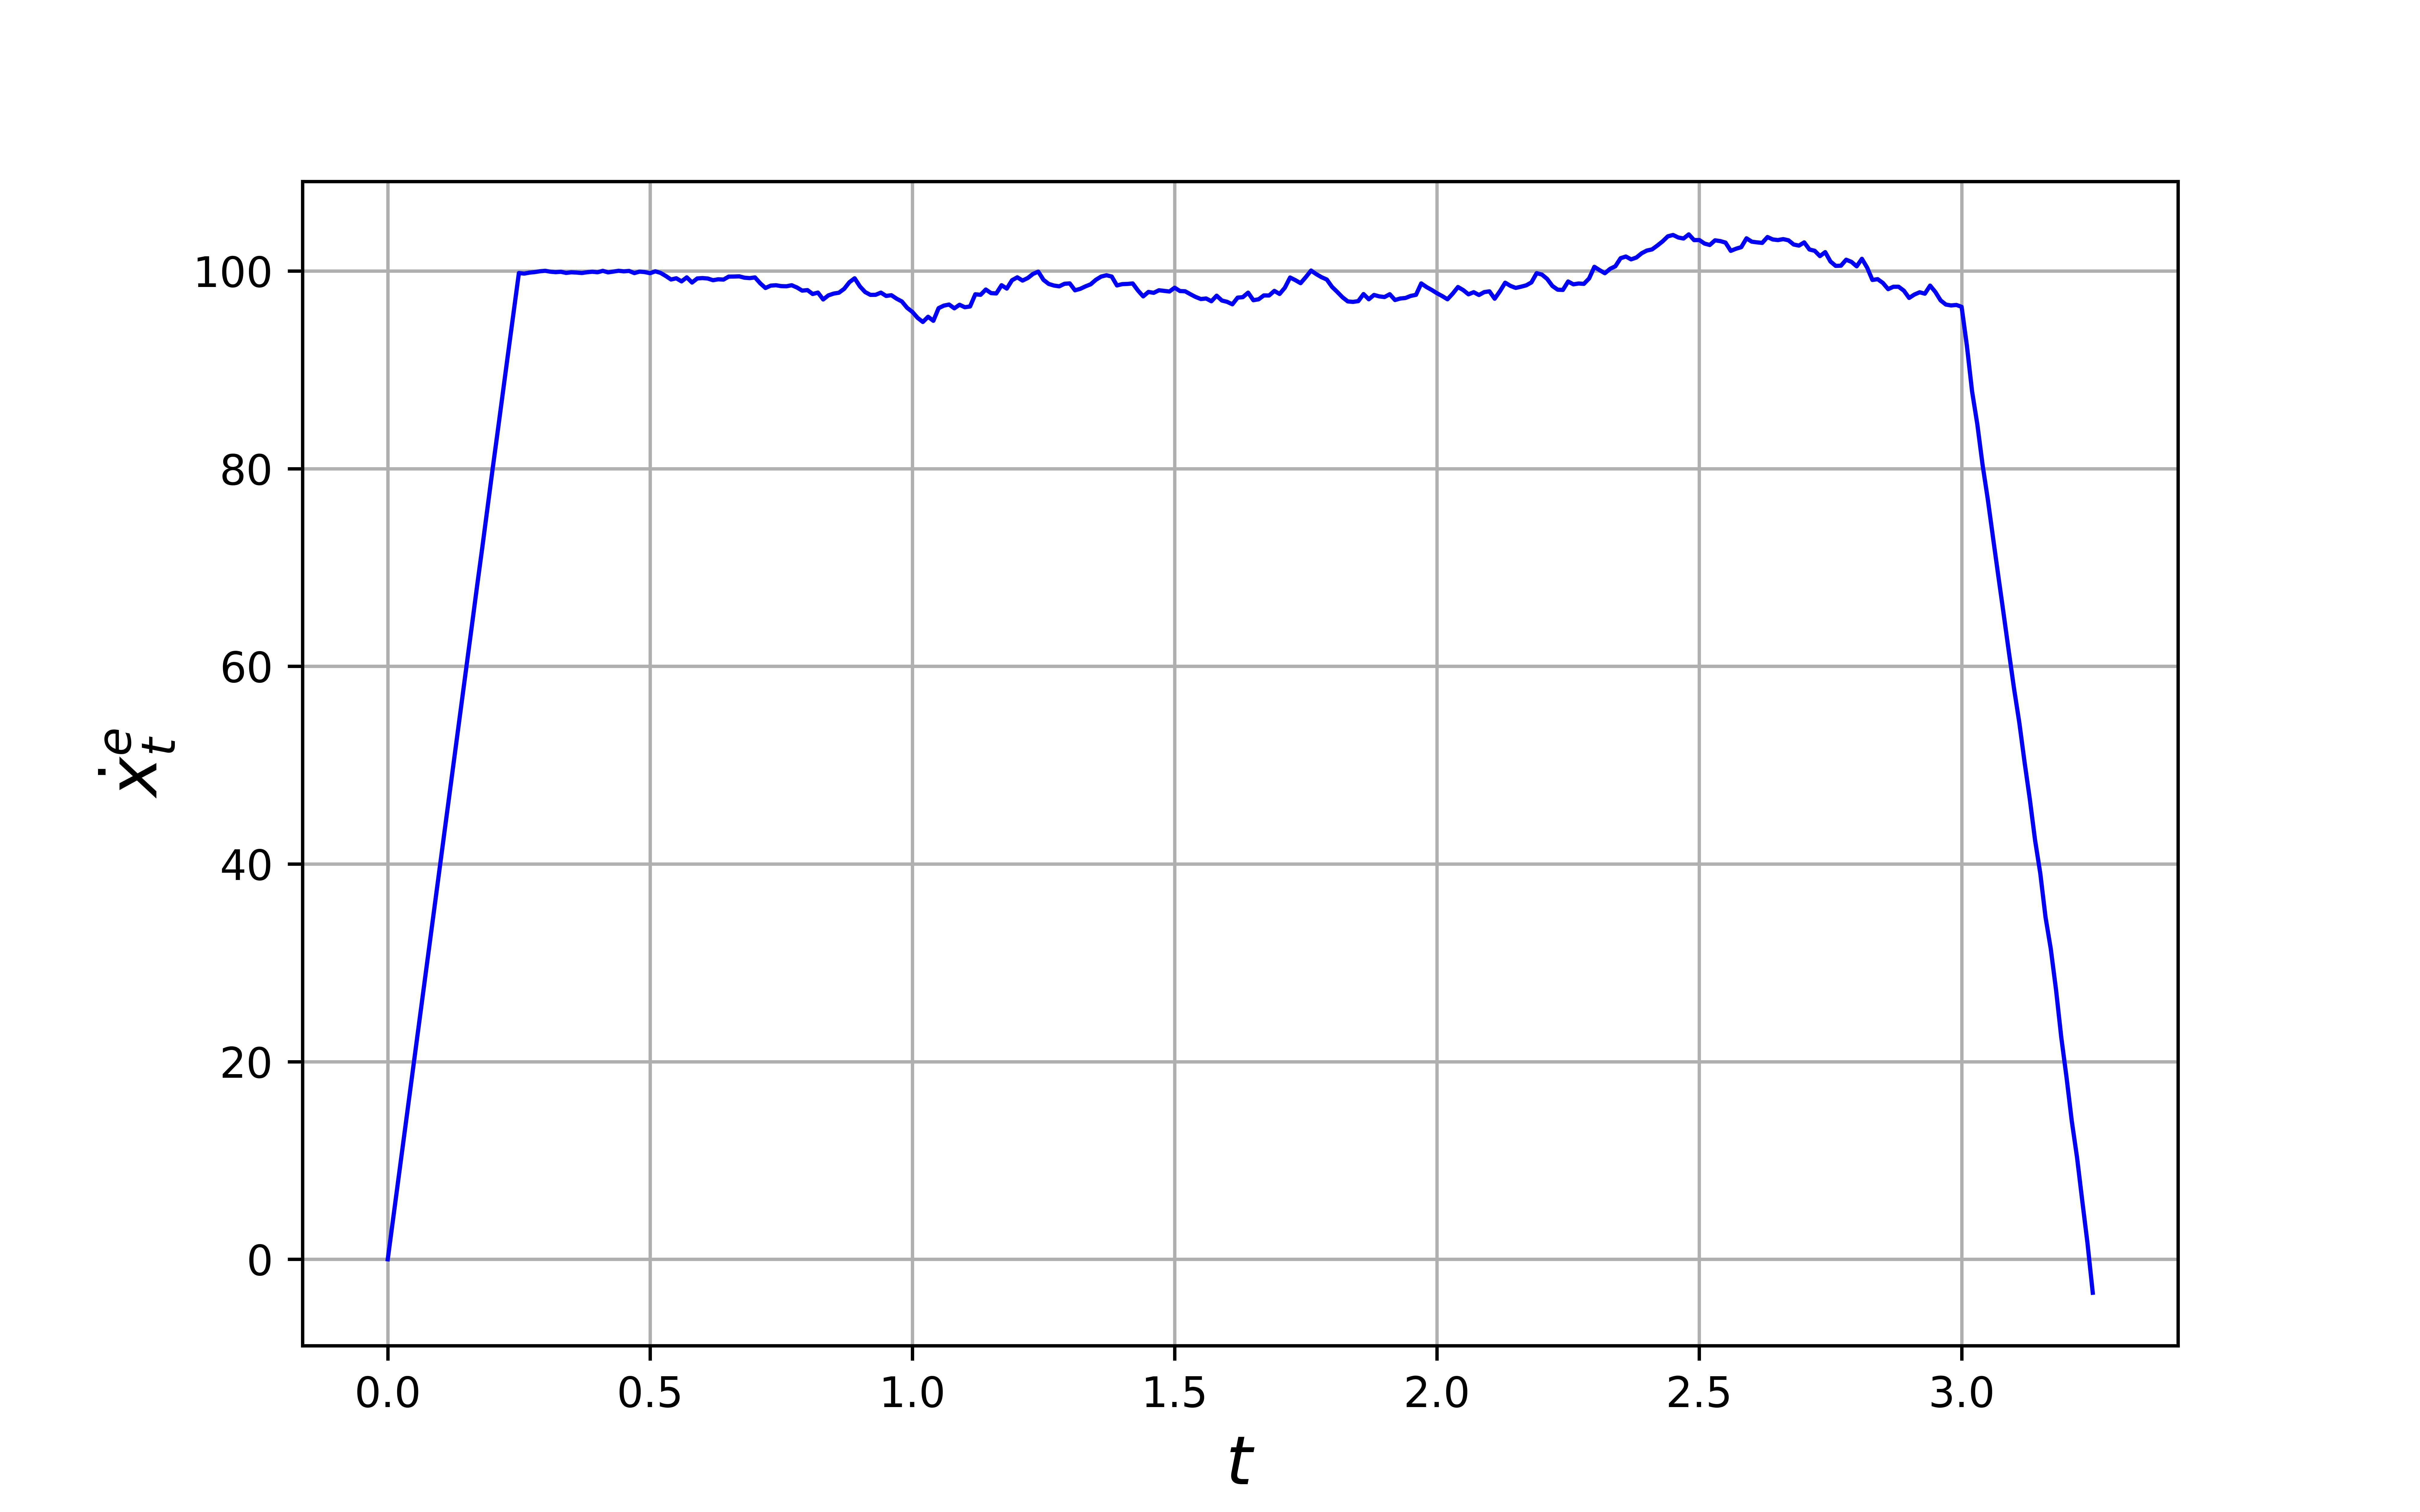
\includegraphics[width=\linewidth]{plots/part1-b.2.png}
        \caption{Estimation $\dot{x}^e_t$ vs $t$}
    \end{minipage}
\end{figure}

\subsection{Kalman Filter Model}
In \nameref{fig:kalman_filter}, $\mu_0 = [0 \ \  0]^T, \Sigma_0 = 10^{-4}I_2$ is the initial belief. Values of $A_t, B_t, R_t, C_t, Q_t$ have been given in \nameref{sec:kinematics_train}.
\begin{figure}[h]
    \centering
    \fbox{
        \begin{minipage}{0.9\linewidth}
        \textbf{Algorithm} \texttt{Kalman\_filter}$(\mu_{t-1}, \Sigma_{t-1}, u_t, z_t)$\\
        \textbf{Prediction Step}\\  
        $\bar{\mu}_t = A_t \mu_{t-1} + B_t u_t$\\  
        $\bar{\Sigma}_t = A_t \Sigma_{t-1} A_t^T + R_t$\\  
        \textbf{Update Step}\\
        $K_t = \bar{\Sigma}_t C_t^T (C_t \bar{\Sigma}_t C_t^T + Q_t)^{-1}$\\
        $\mu_t = \bar{\mu}_t + K_t (z_t - C_t \bar{\mu}_t)$\\
        $ \Sigma_t = (I - K_t C_t) \bar{\Sigma}_t$\\ 
        \textbf{return} $\mu_t, \Sigma_t$\\
        \end{minipage}
    }
    \caption{Kalman Filter Algorithm}
    \label{fig:kalman_filter}
\end{figure}

\subsection{Uncertainty Bars for $x^e_t$}
In \autoref{fig:uncertainty_bar} we see that the uncertainty bar is very thin initially, but it becomes wider later, possibly due to the error in action the model $R_t$ that keeps getting added in each step. For most of the time, the one-standard-deviation uncertainty band contains the ground truth.
\begin{figure}[H]
    \centering
    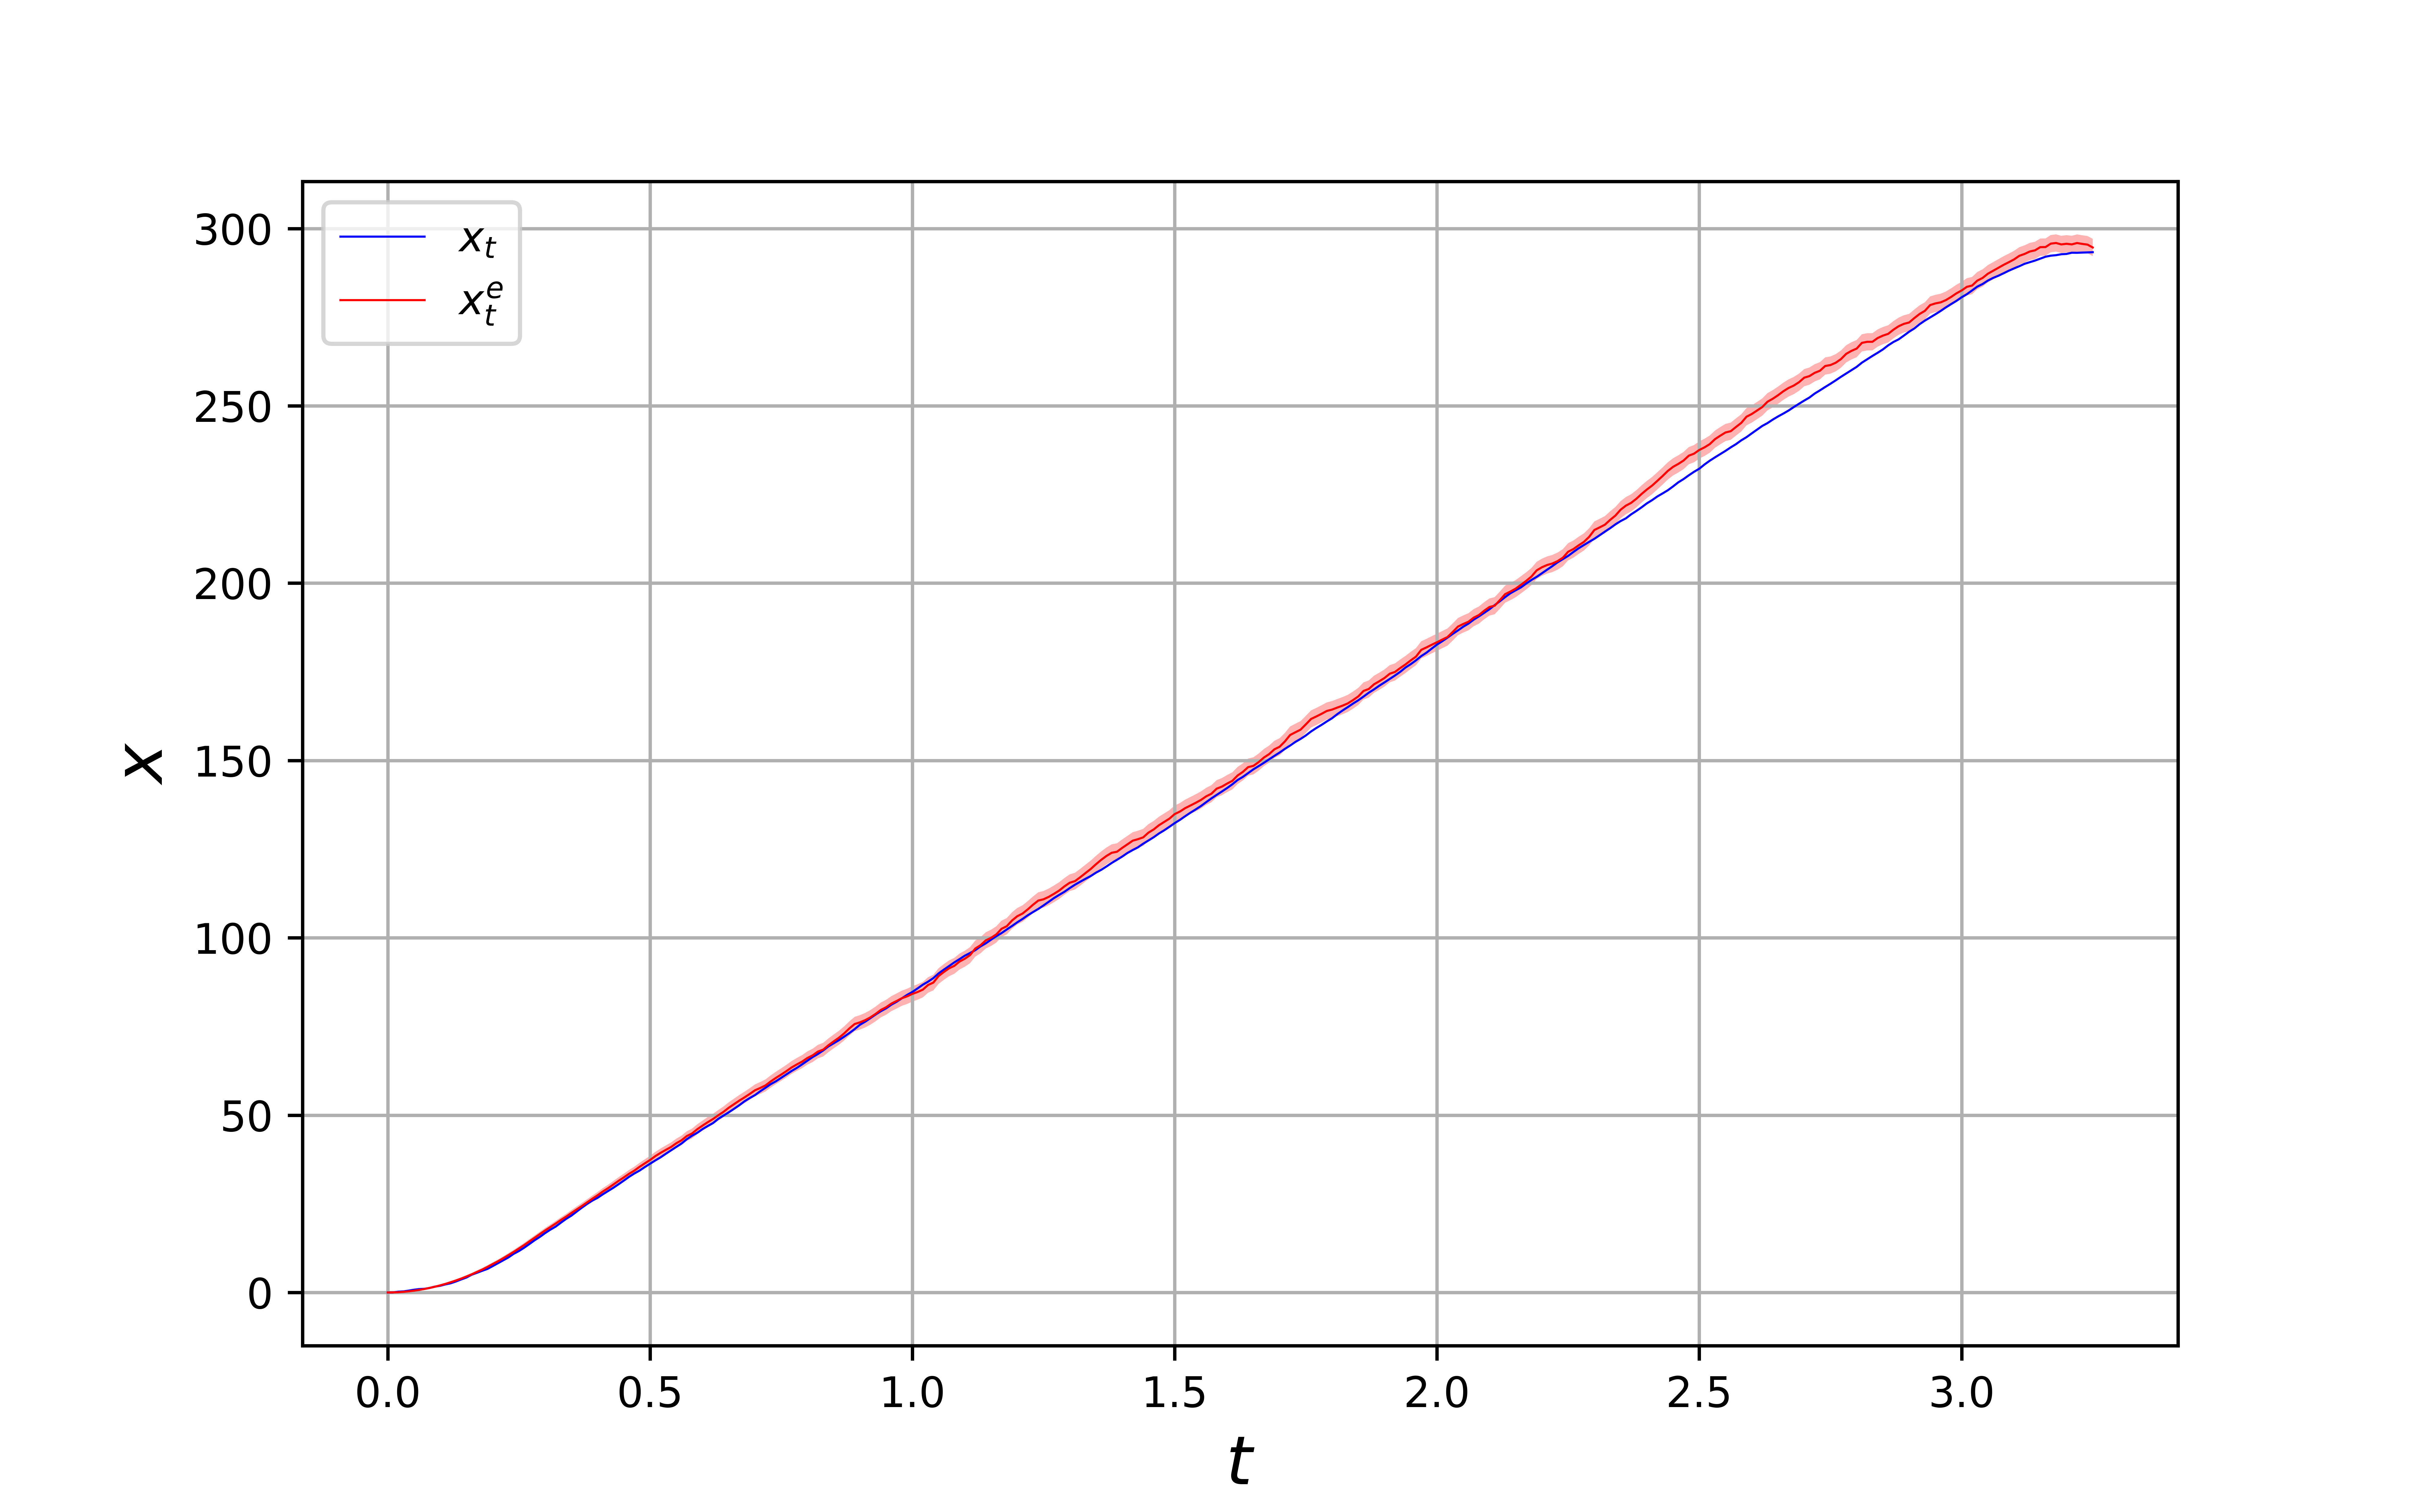
\includegraphics[width=1.0\linewidth]{plots/part1-c.png}
    \caption{$x_t$ and Uncertainty bar of $x_t^e$}
    \label{fig:uncertainty_bar}
\end{figure}

\subsection{Varying $\sigma_x, \sigma_{\dot{x}},
\sigma_s$}
\begin{itemize}
    \item In \autoref{fig:part1-vary-sigma_x}
    The uncertainty band gets wider on increasing $\sigma_x$. Both ground truth and estimated trajectories are affected, as $\sigma_x$ causes noise in the motion model. 
    
\item In \autoref{fig:part1-vary-sigma_x_dot}, both ground truth and estimated trajectories with $\sigma_{\dot{x}} = 5.0$ are significantly different from those with lower $\sigma_{\dot{x}}$. This is because $\sigma_{\dot{x}}$ directly affects the noise in the motion model. The uncertainty band becomes wider, and there are many more fluctuations as $\sigma_{\dot{x}}$ is increased.

 
    \item \autoref{fig:part1-vary-sigma_s} shows, on changing $\sigma_s$ there's nearly no variation in $x_t$ as the ground truth does not use observations. The difference is only due to the random noise in the motion model. In $x_t^e$, the uncertainty band clearly becomes wider as $\sigma_s$ increases. As observation is the only part in Kalman Filter where the belief variance reduces. The trajectories themselves, however, are not very different (varying $\sigma_s$) compared to the earlier parts (causing noise in the motion model).
\end{itemize}
\begin{figure}[H]
    \centering
    \begin{minipage}{0.491\linewidth}
        \centering
        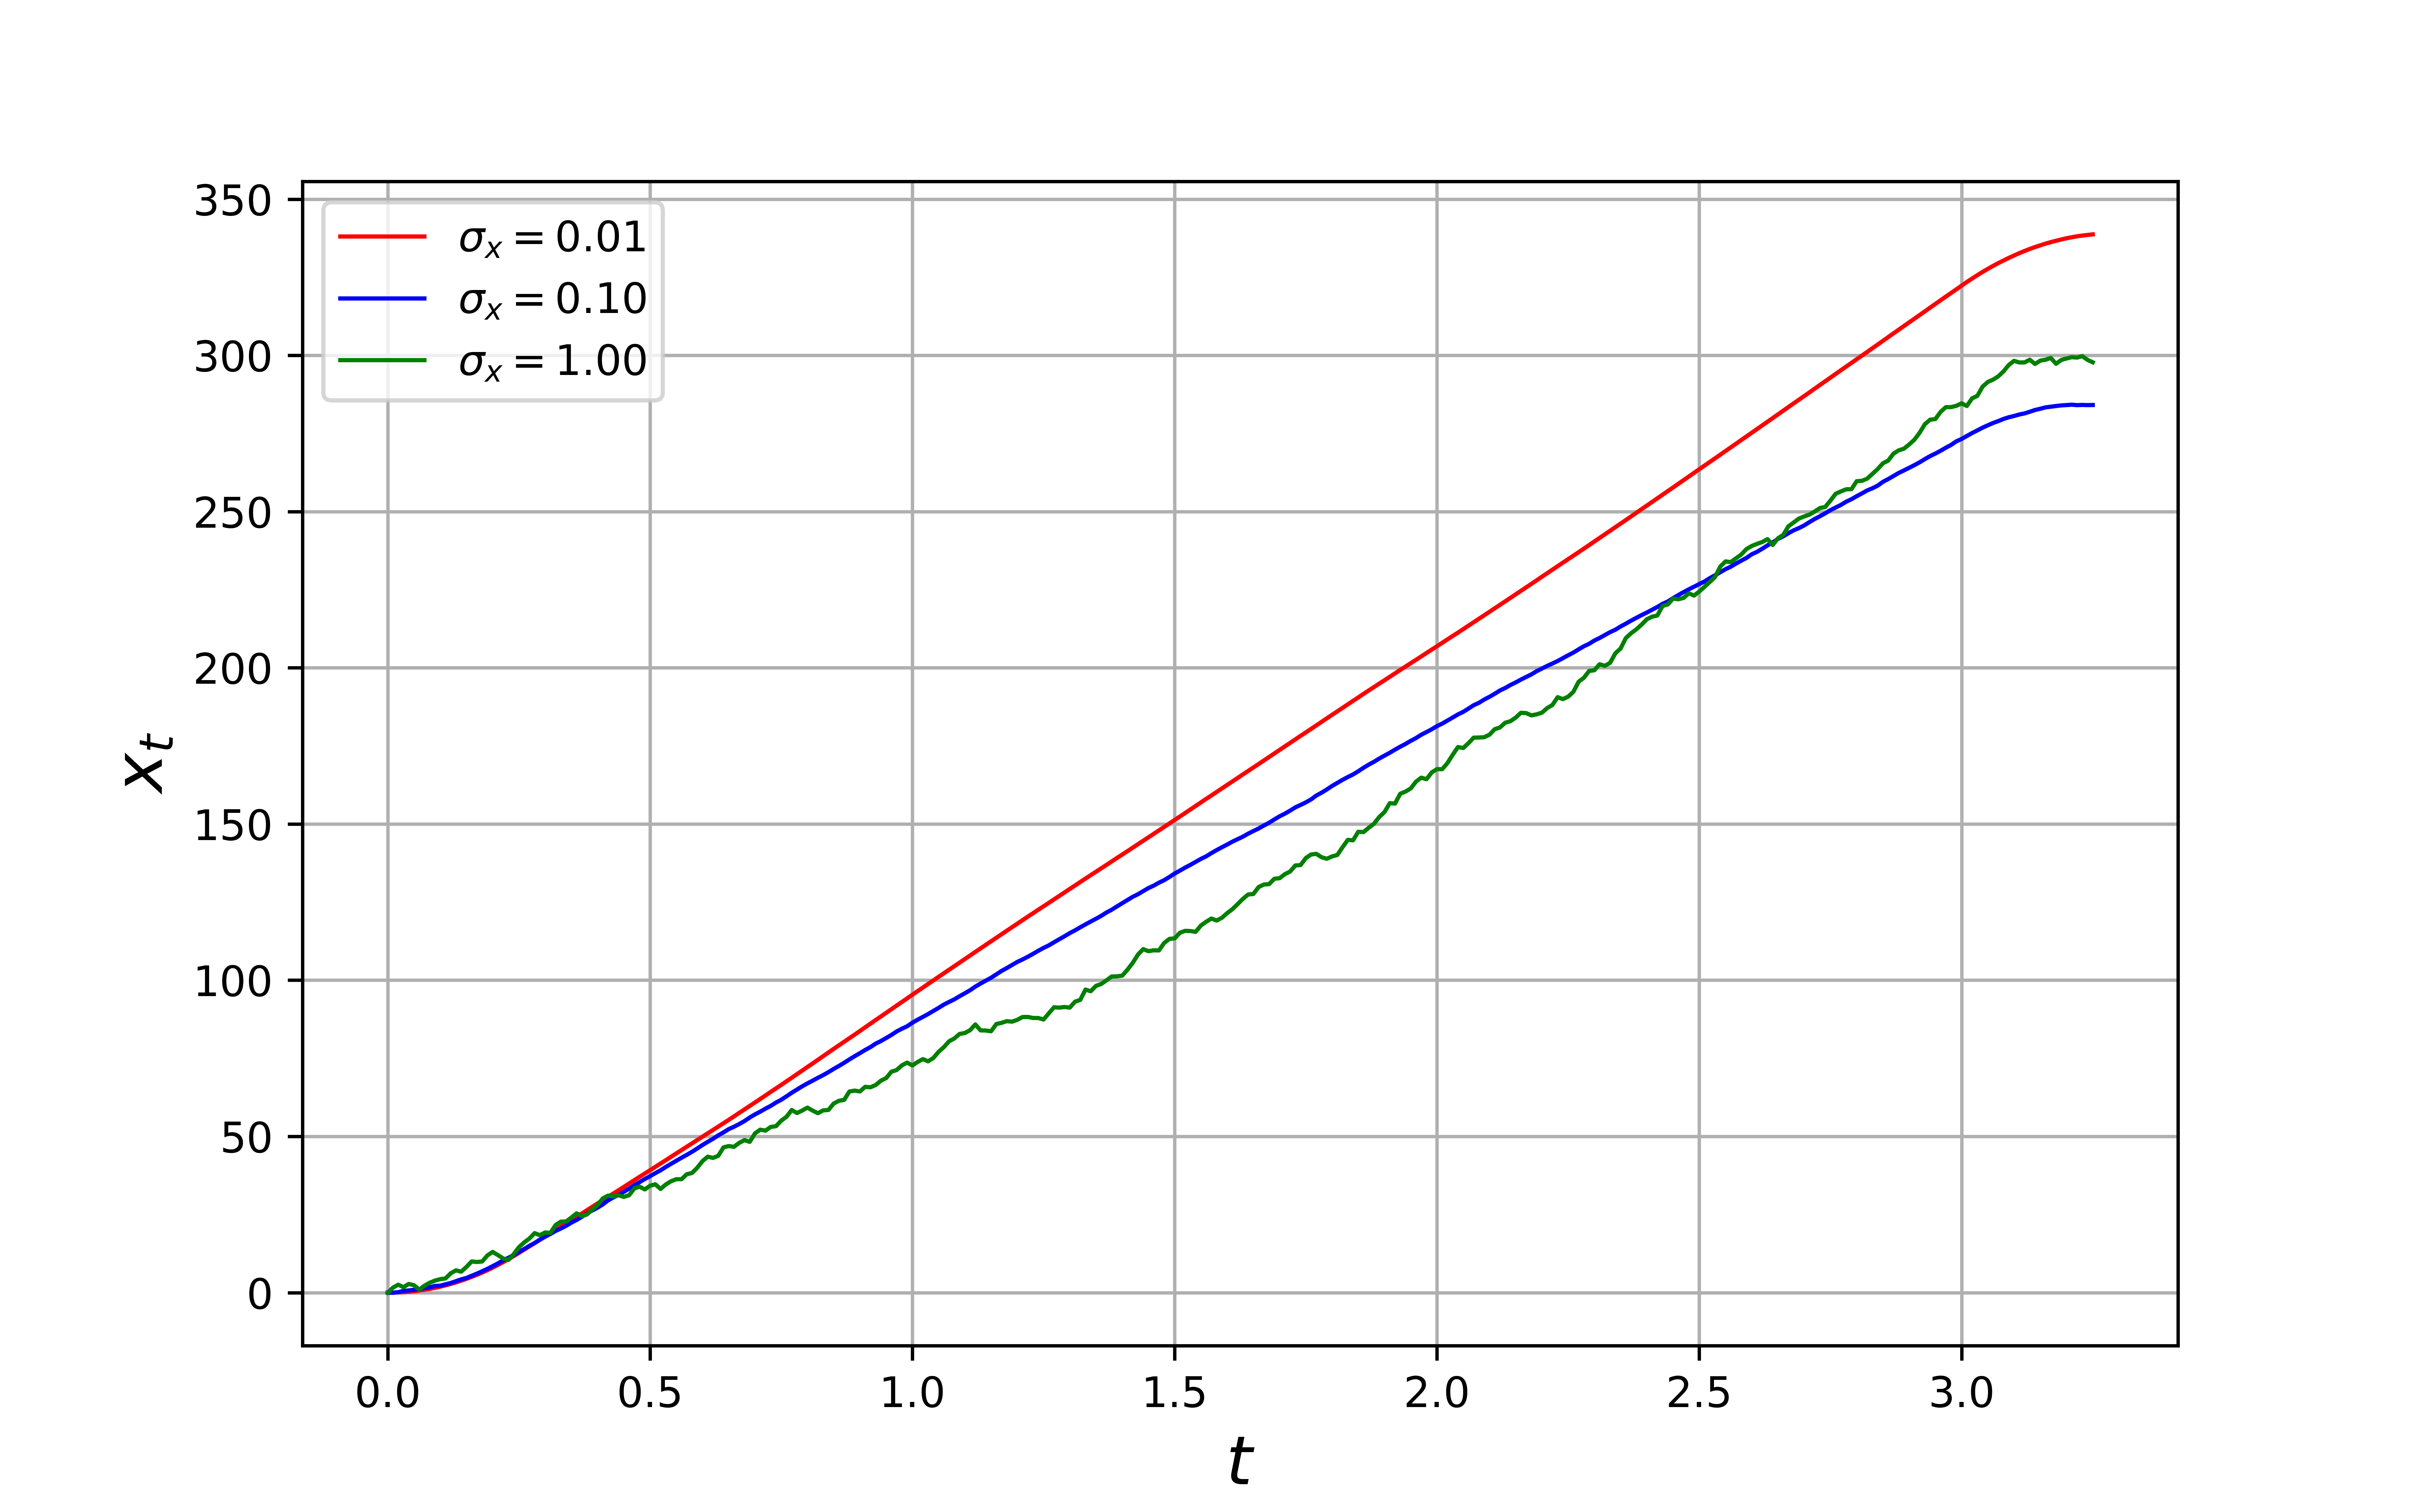
\includegraphics[width=\linewidth]{plots/part1-d.0-xt.png}
        \caption*{$x_t$ vs $t$}
    \end{minipage}
    \hfill
    \begin{minipage}{0.49\linewidth}
        \centering
        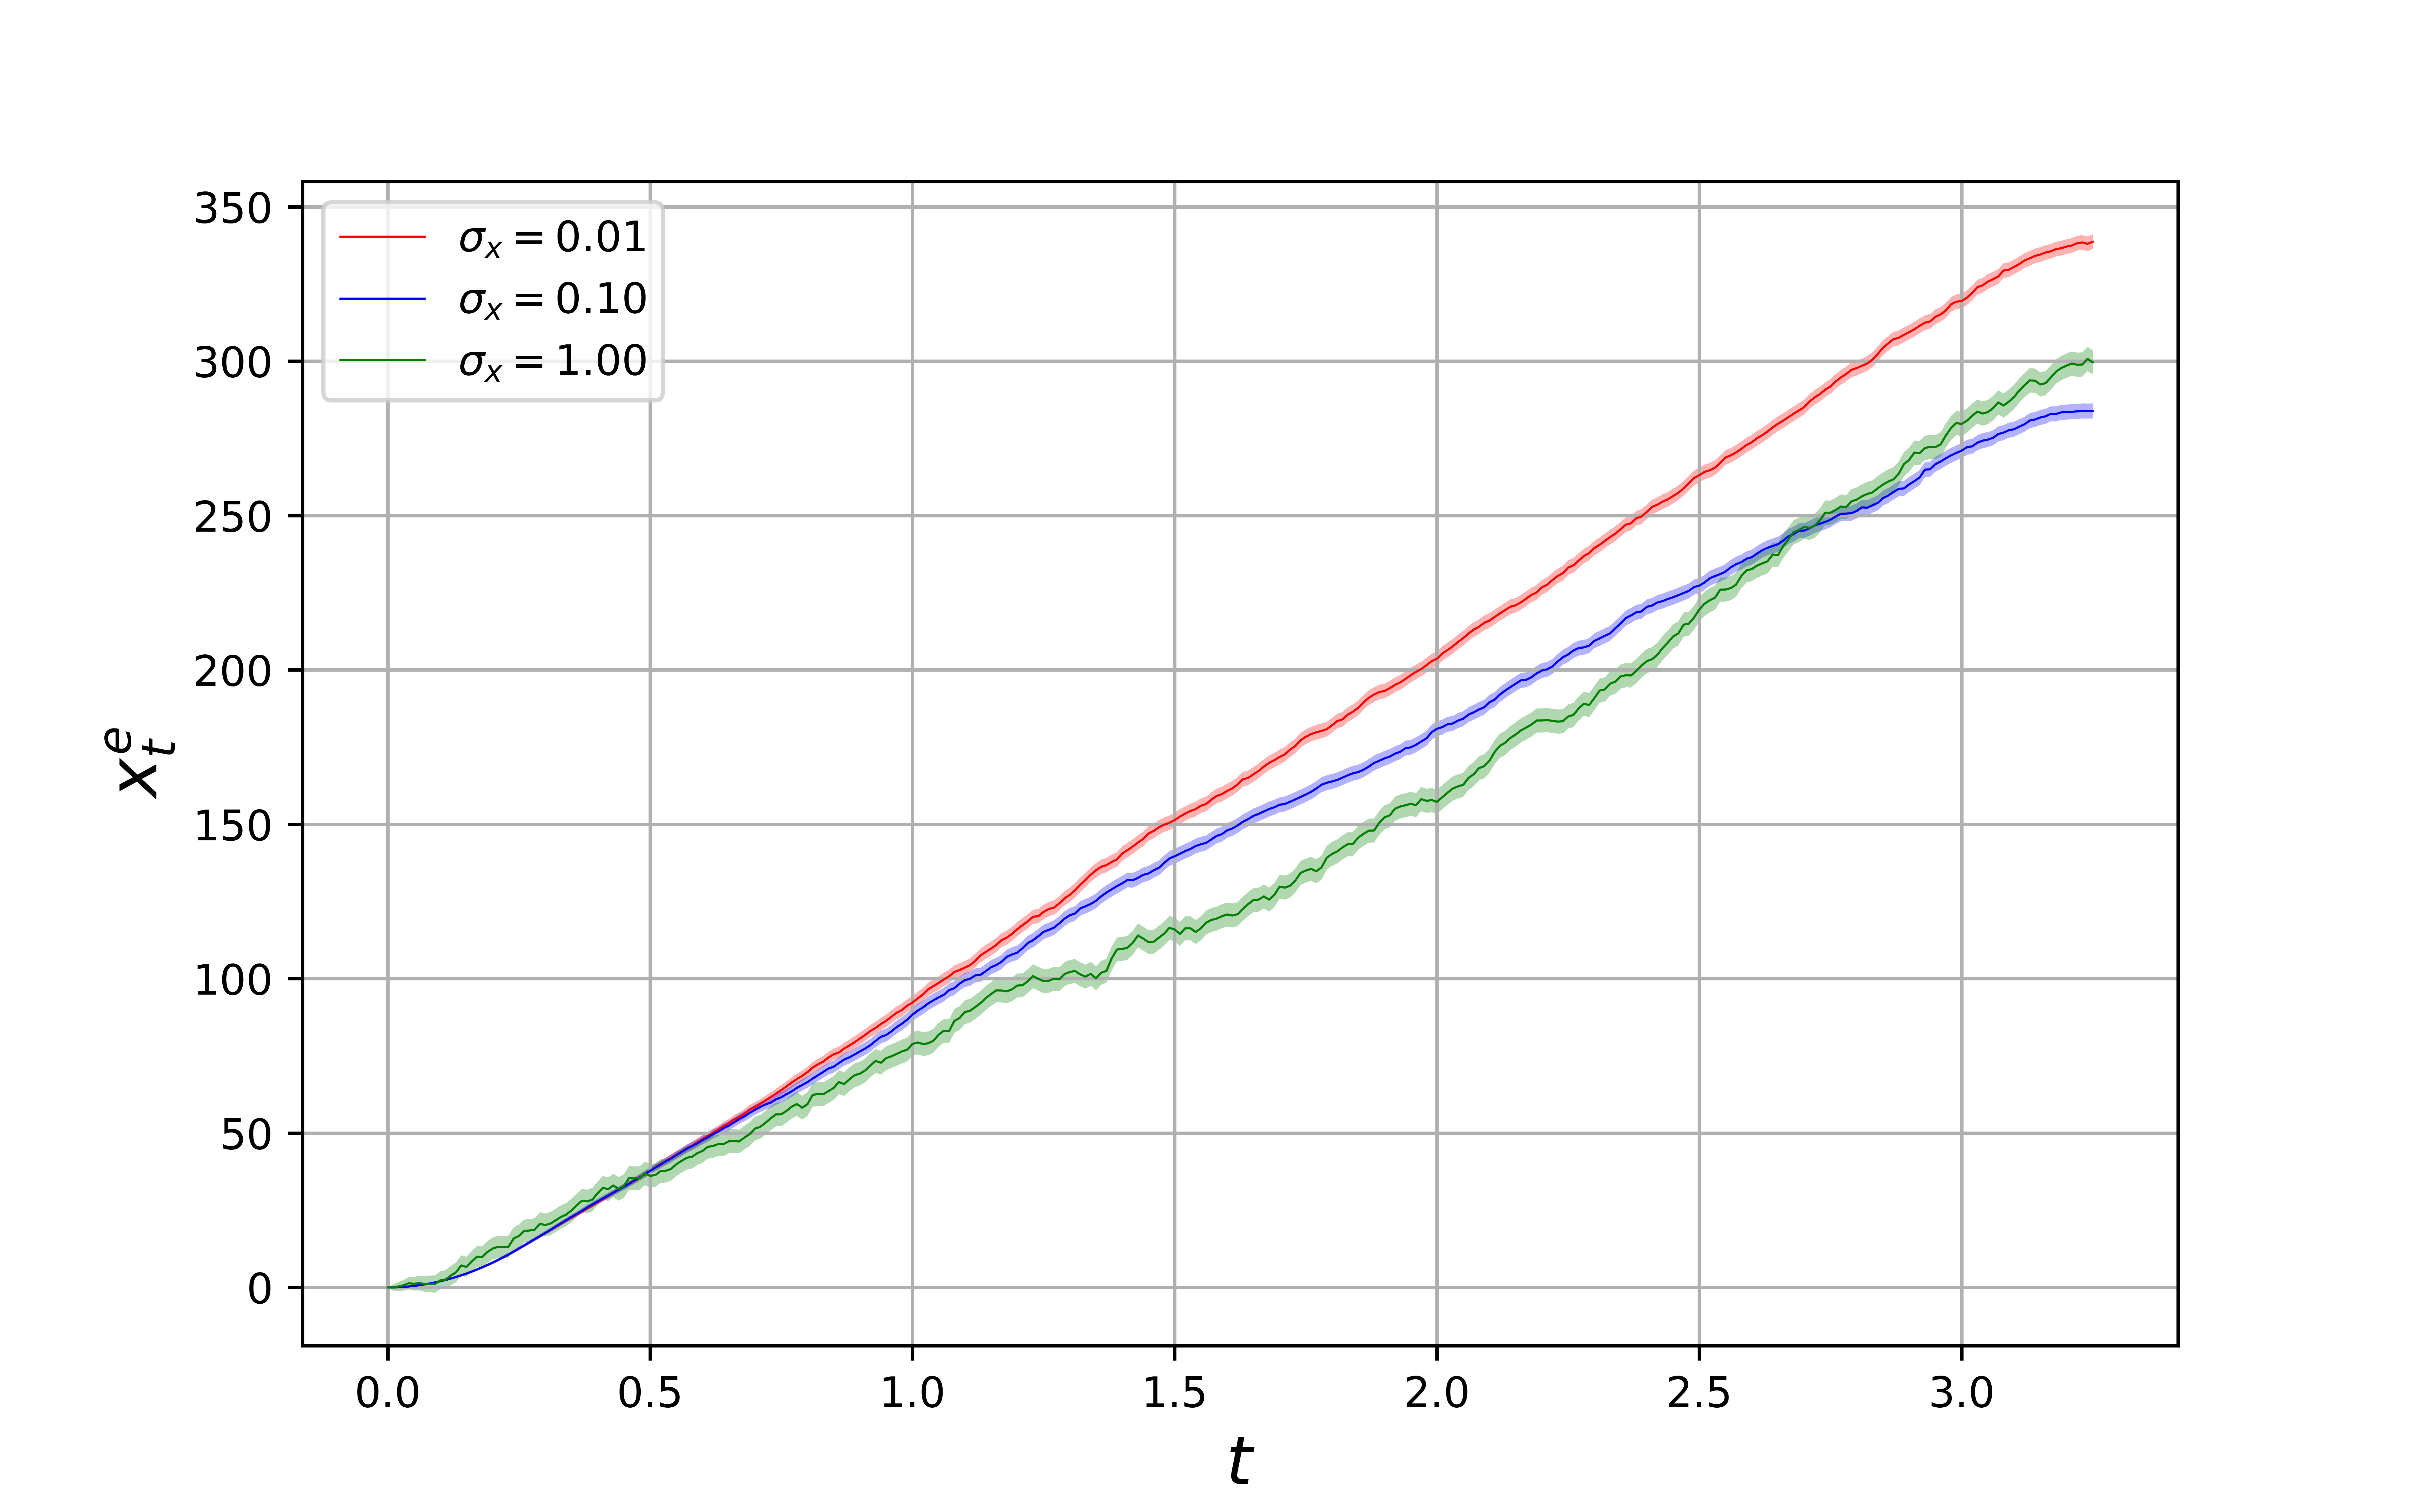
\includegraphics[width=\linewidth]{plots/part1-d.0-xe.png}
         \caption*{$x_t^e$ vs $t$}
    \end{minipage}
    \caption{Varying $\sigma_x = 0.01, 0.1, 1.0$}
    \label{fig:part1-vary-sigma_x}
\end{figure}
\begin{figure}[H]
    \centering
    \begin{minipage}{0.491\linewidth}
        \centering
        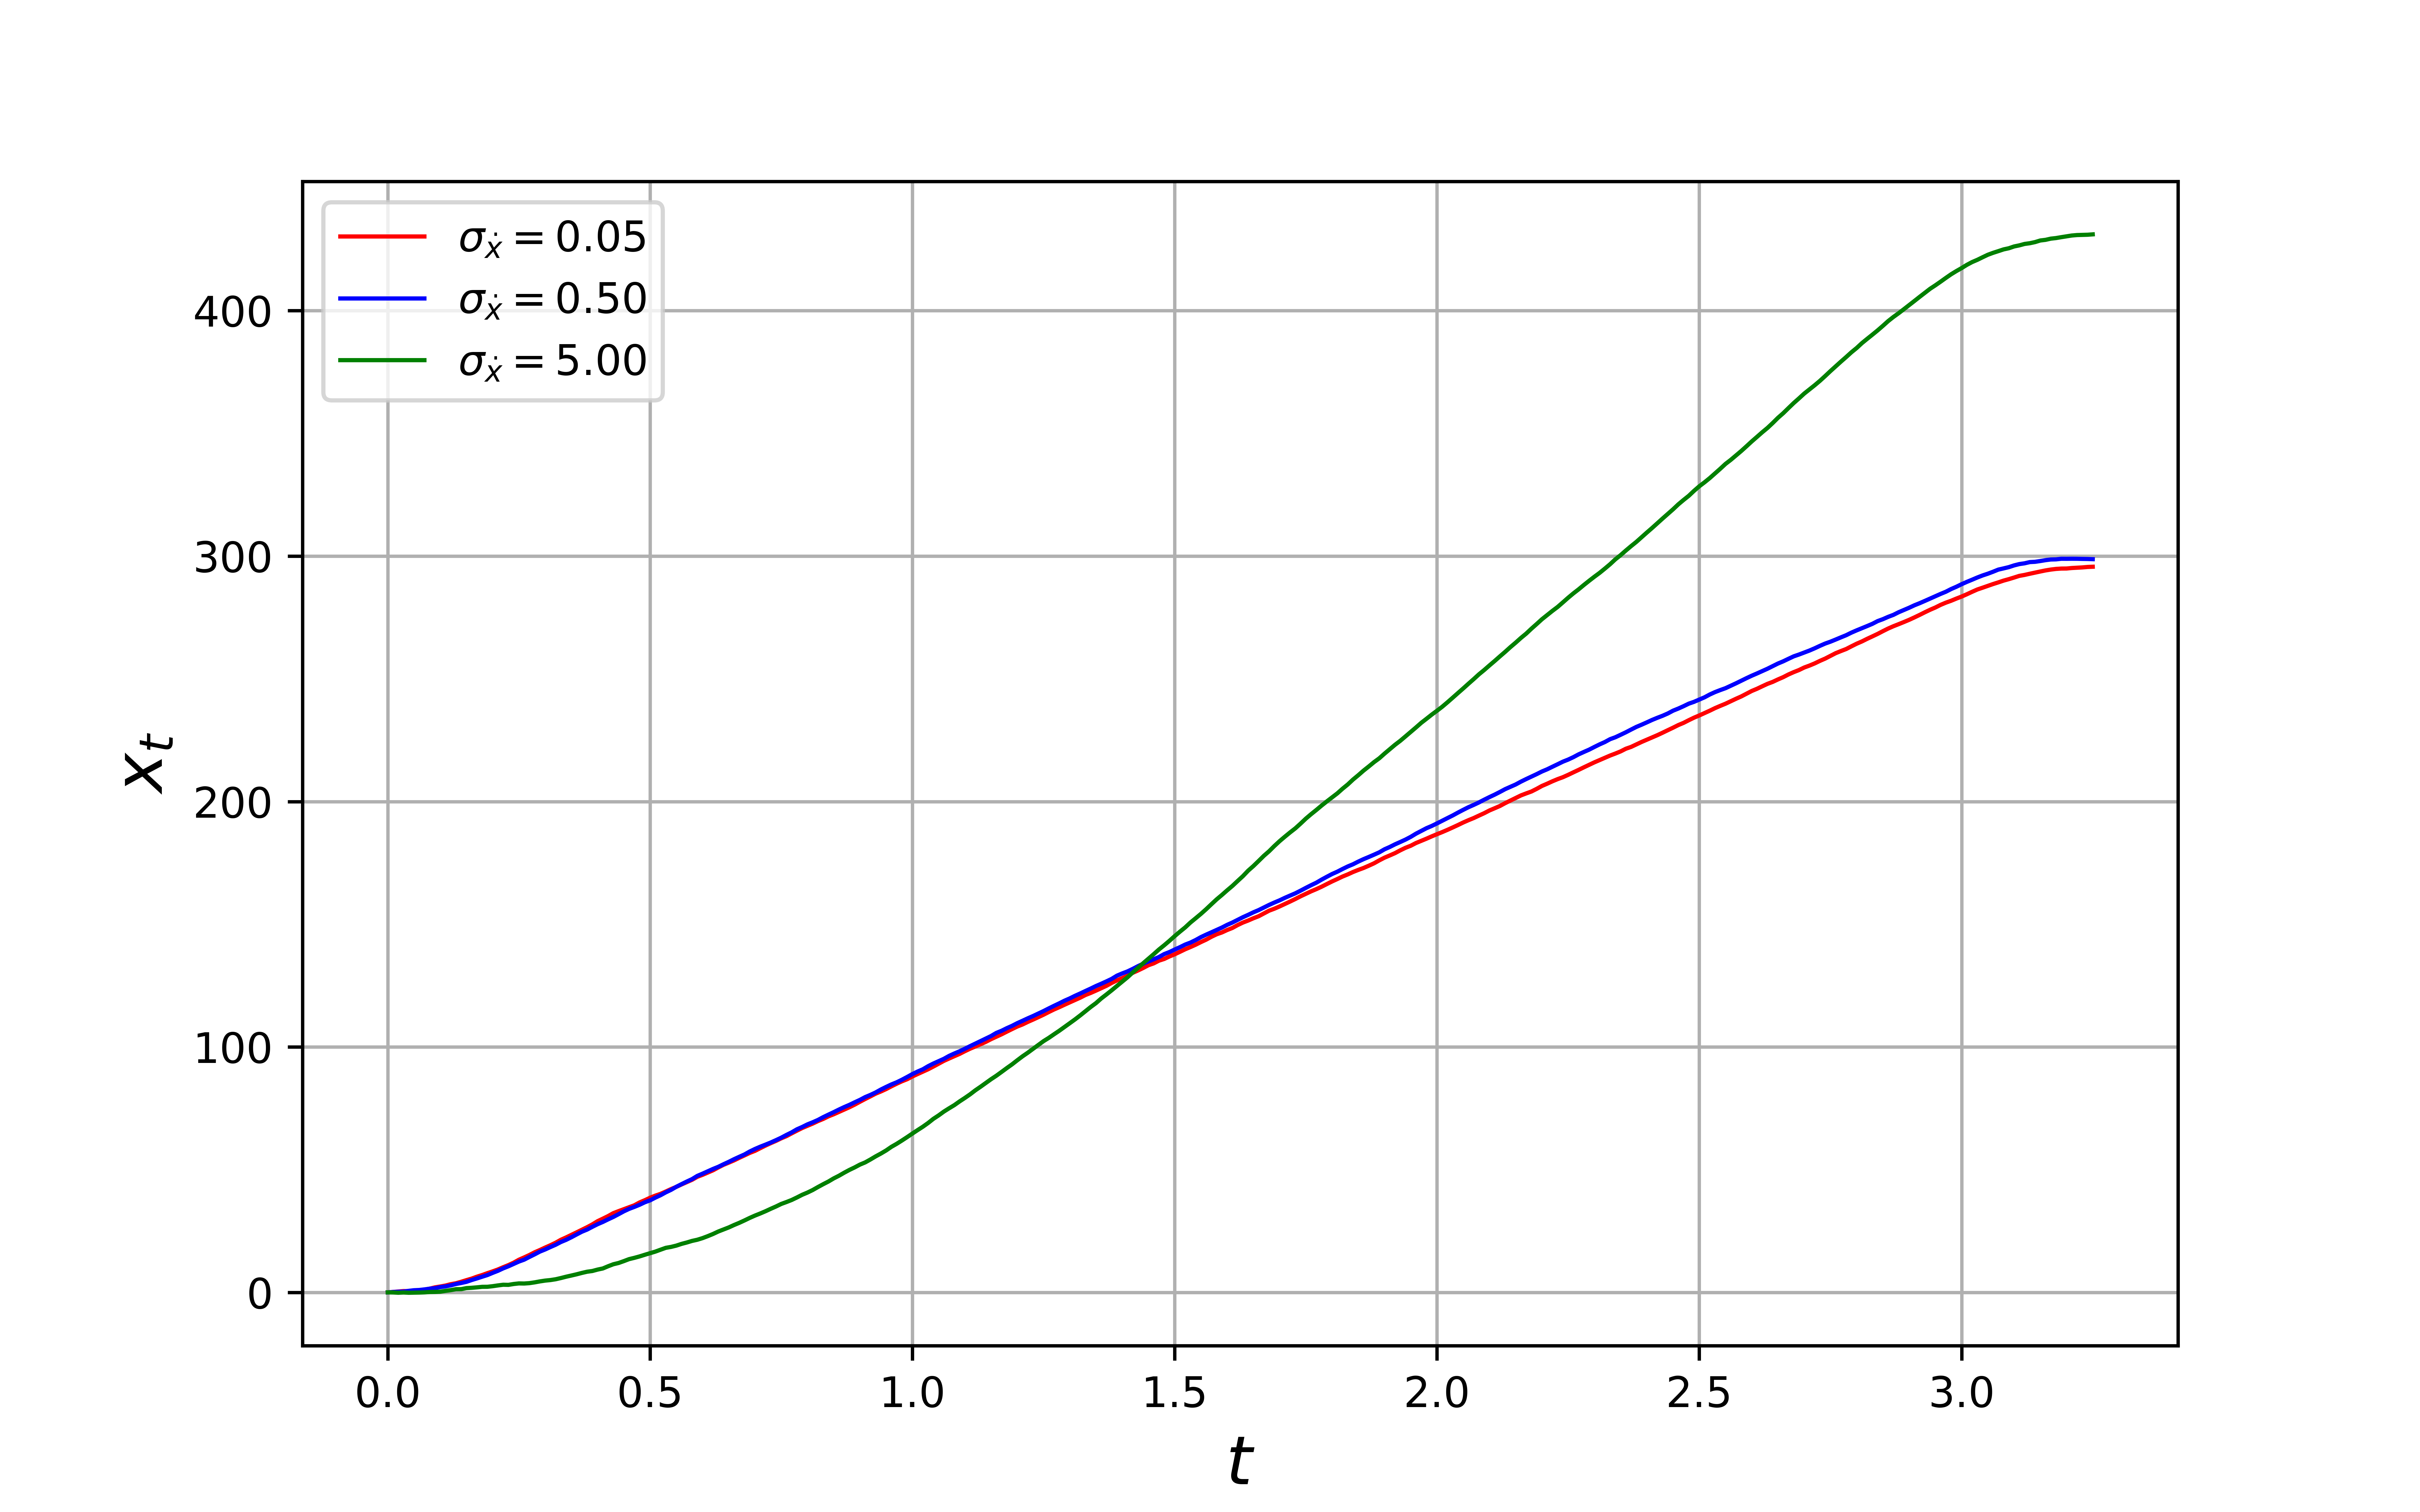
\includegraphics[width=\linewidth]{plots/part1-d.1-xt.png}
        \caption*{$x_t$ vs $t$}

    \end{minipage}
    \hfill
    \begin{minipage}{0.49\linewidth}
        \centering
        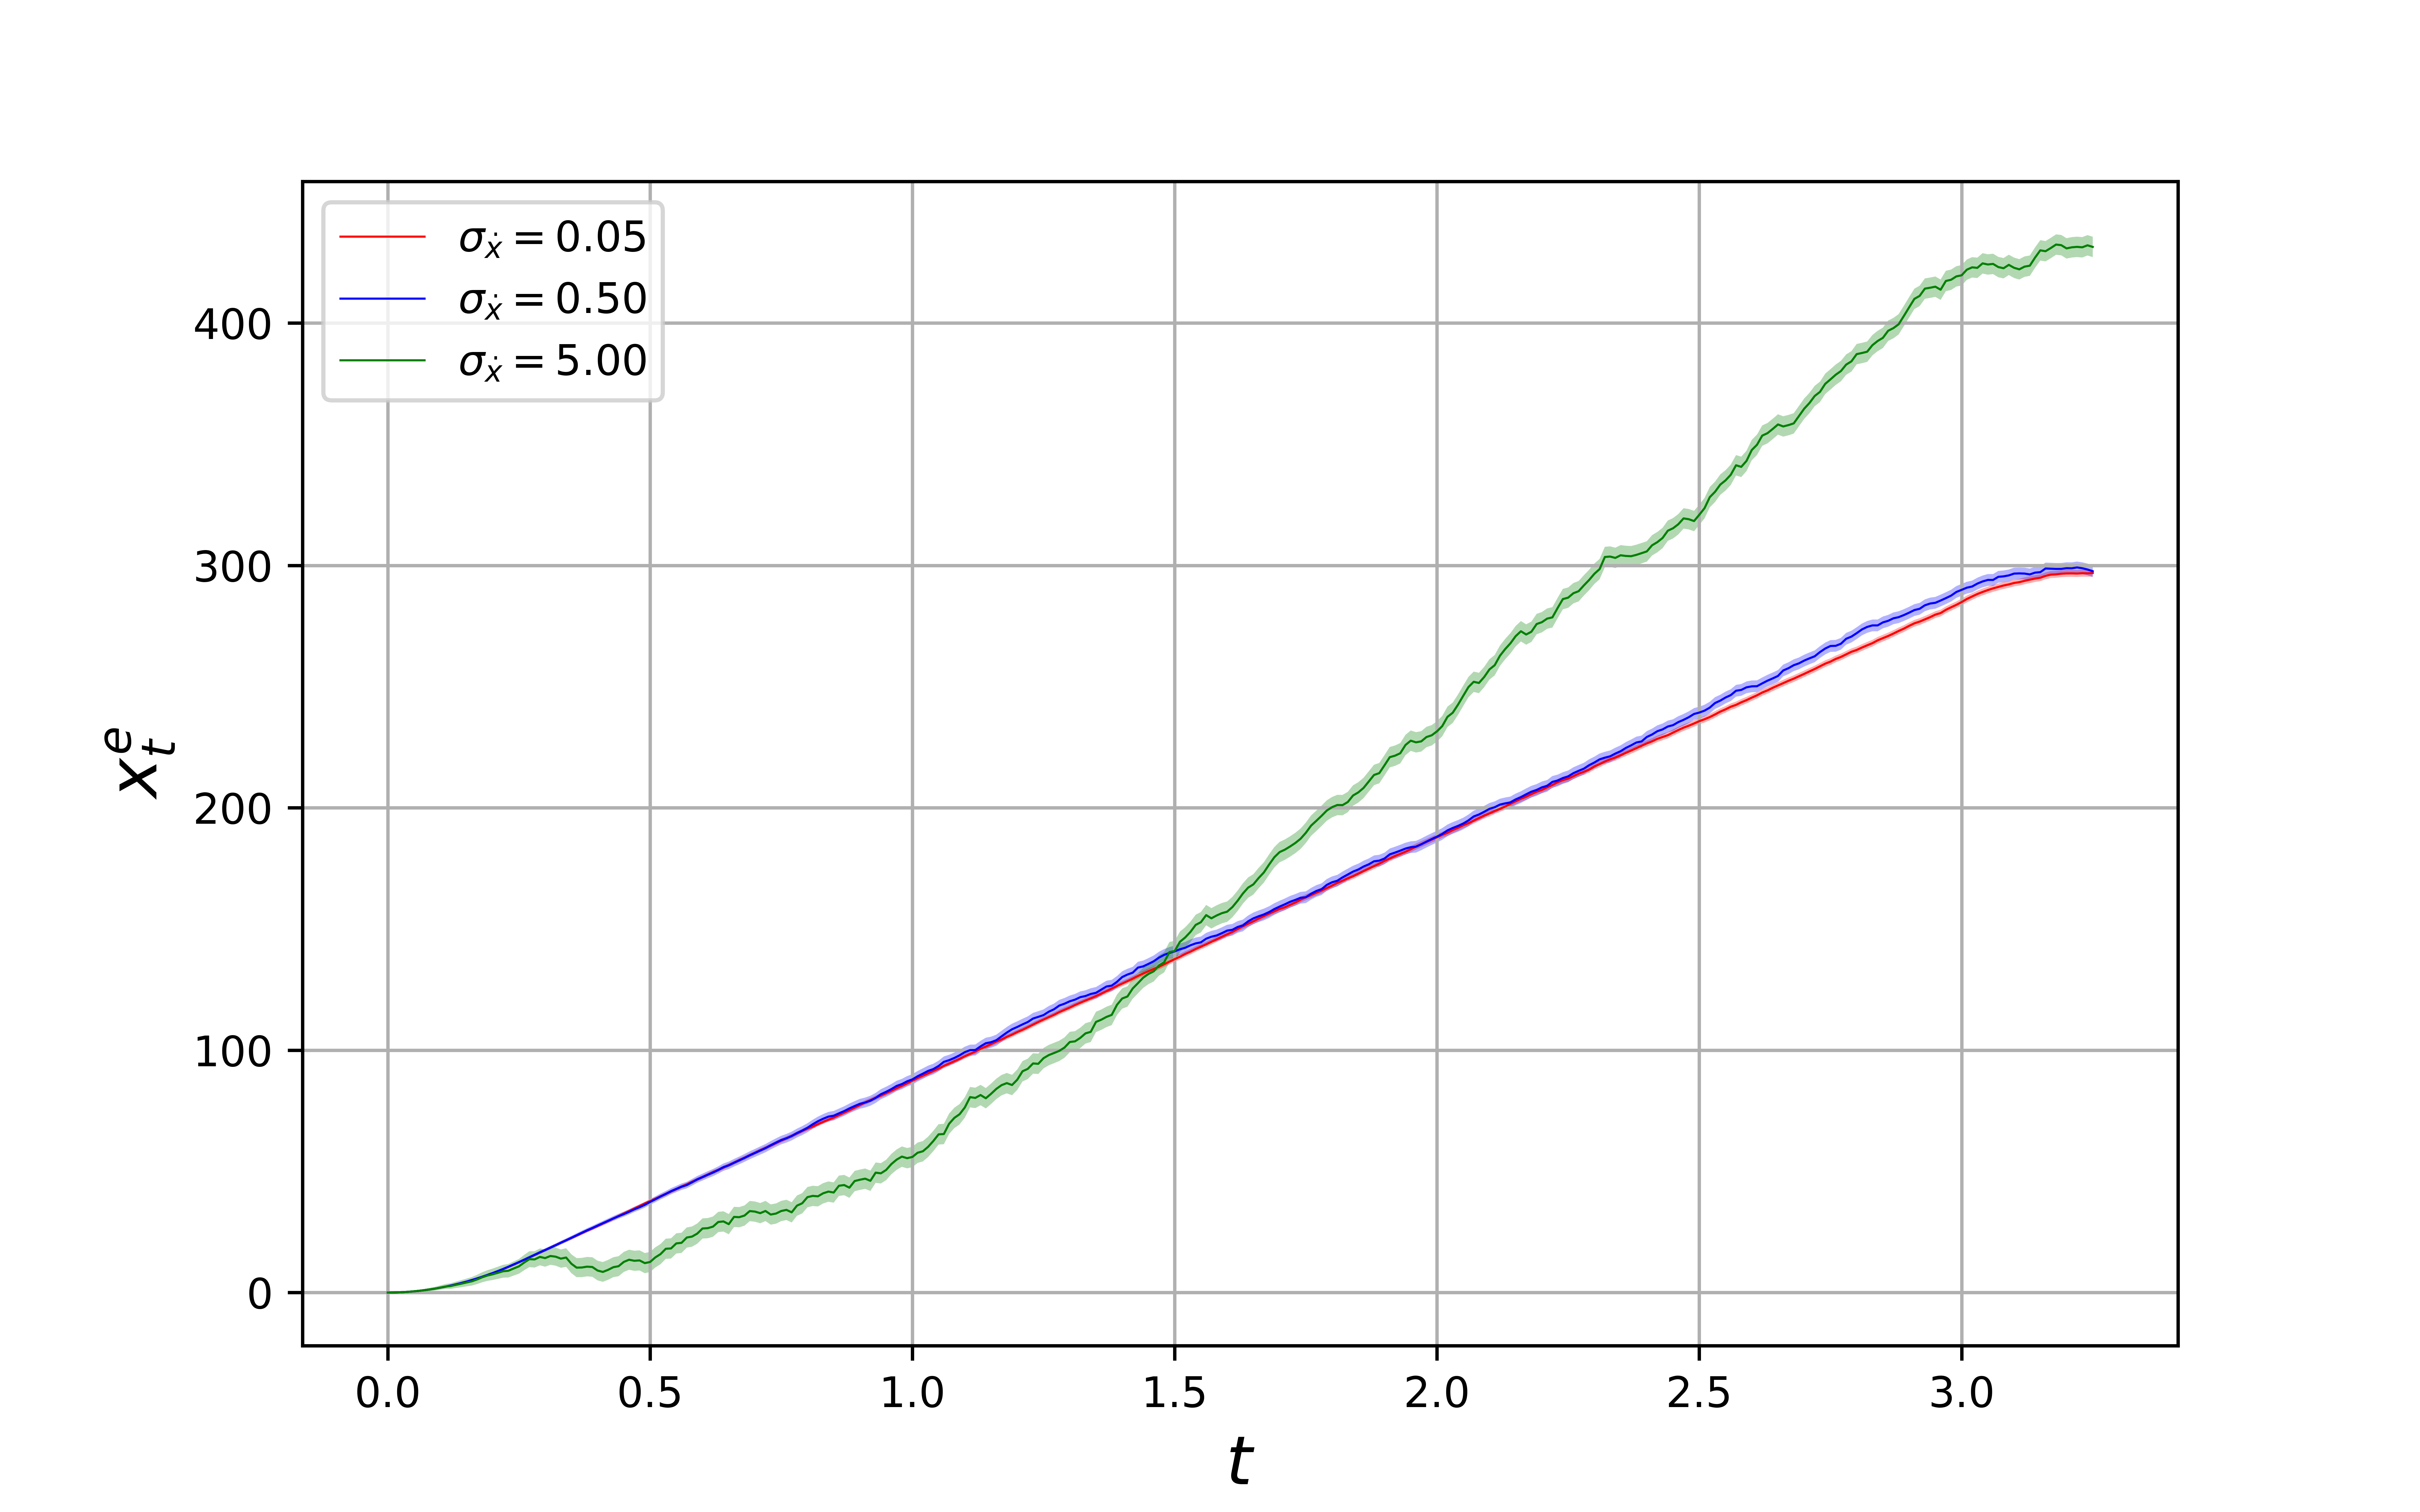
\includegraphics[width=\linewidth]{plots/part1-d.1-xe.png}
         \caption*{$x_t^e$ vs $t$}
    \end{minipage}
    \caption{Varying $\sigma_{\dot{x}} = 0.05, 0.5, 5.0$}
    \label{fig:part1-vary-sigma_x_dot}
    
\end{figure}

\begin{figure}[H]
    \centering
    \begin{minipage}{0.49\linewidth}
        \centering
        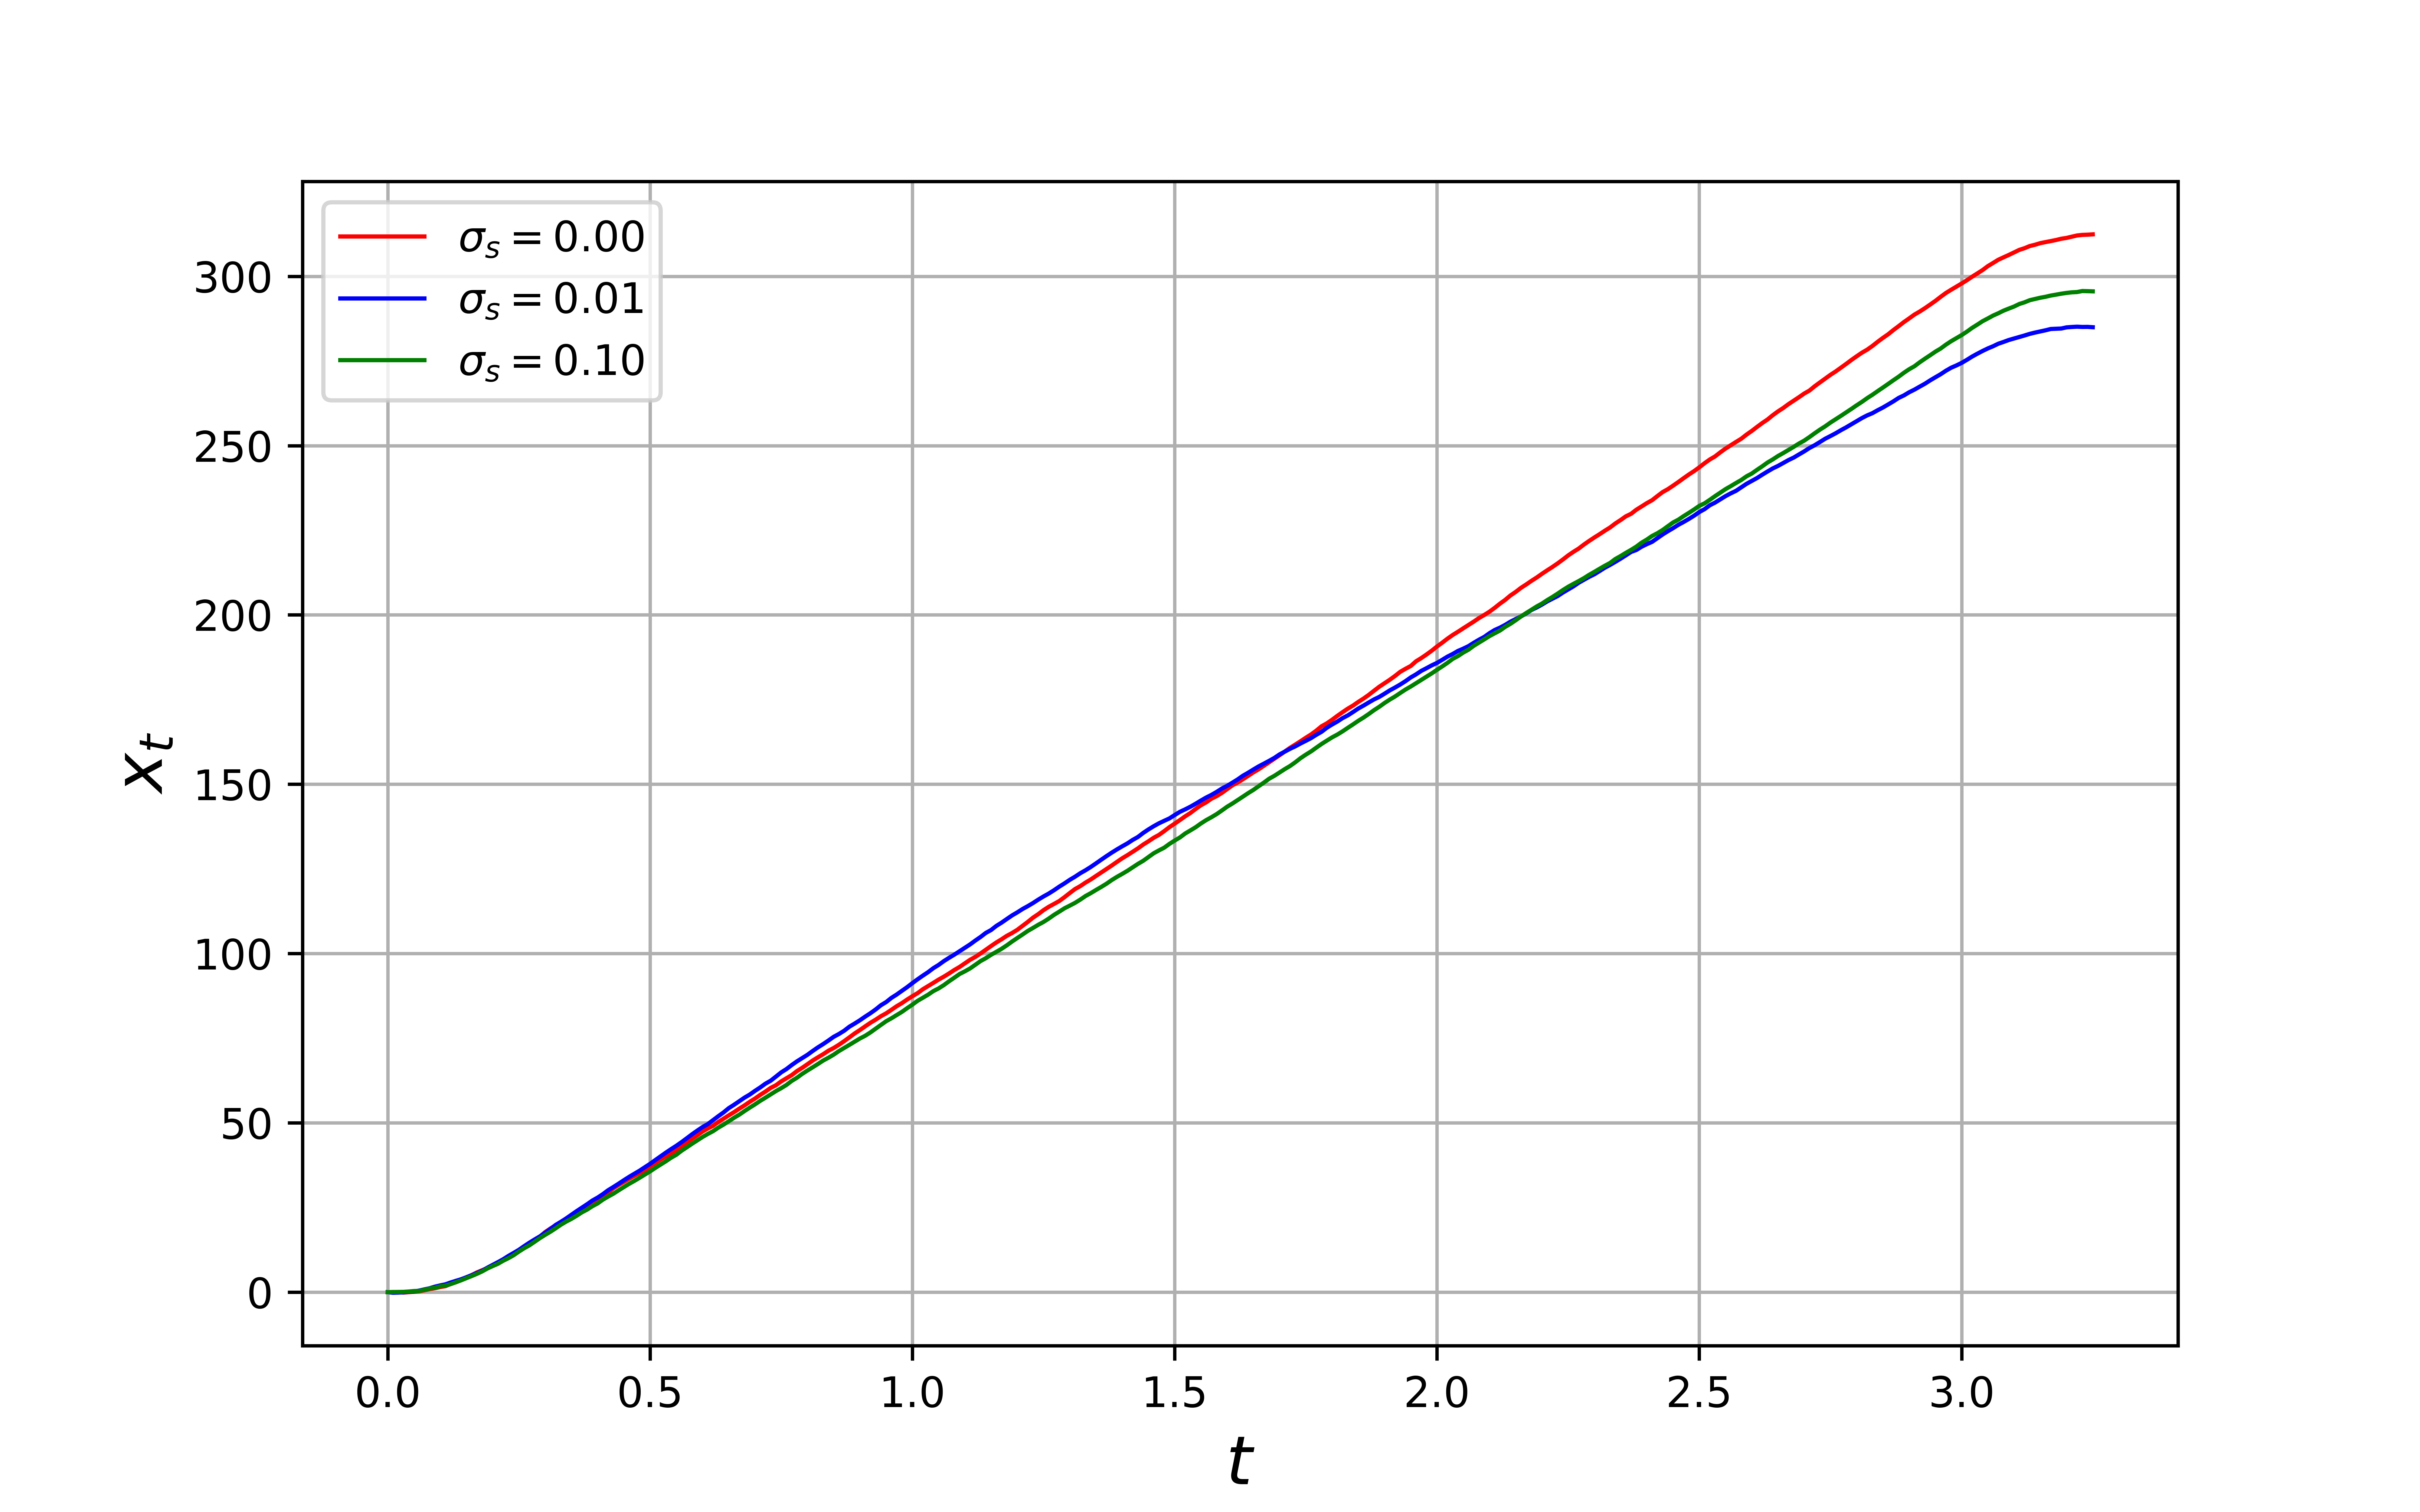
\includegraphics[width=\linewidth]{plots/part1-d.2-xt.png}
        \caption*{$x_t$ vs $t$}

    \end{minipage}
    \hfill
    \begin{minipage}{0.49\linewidth}
        \centering
        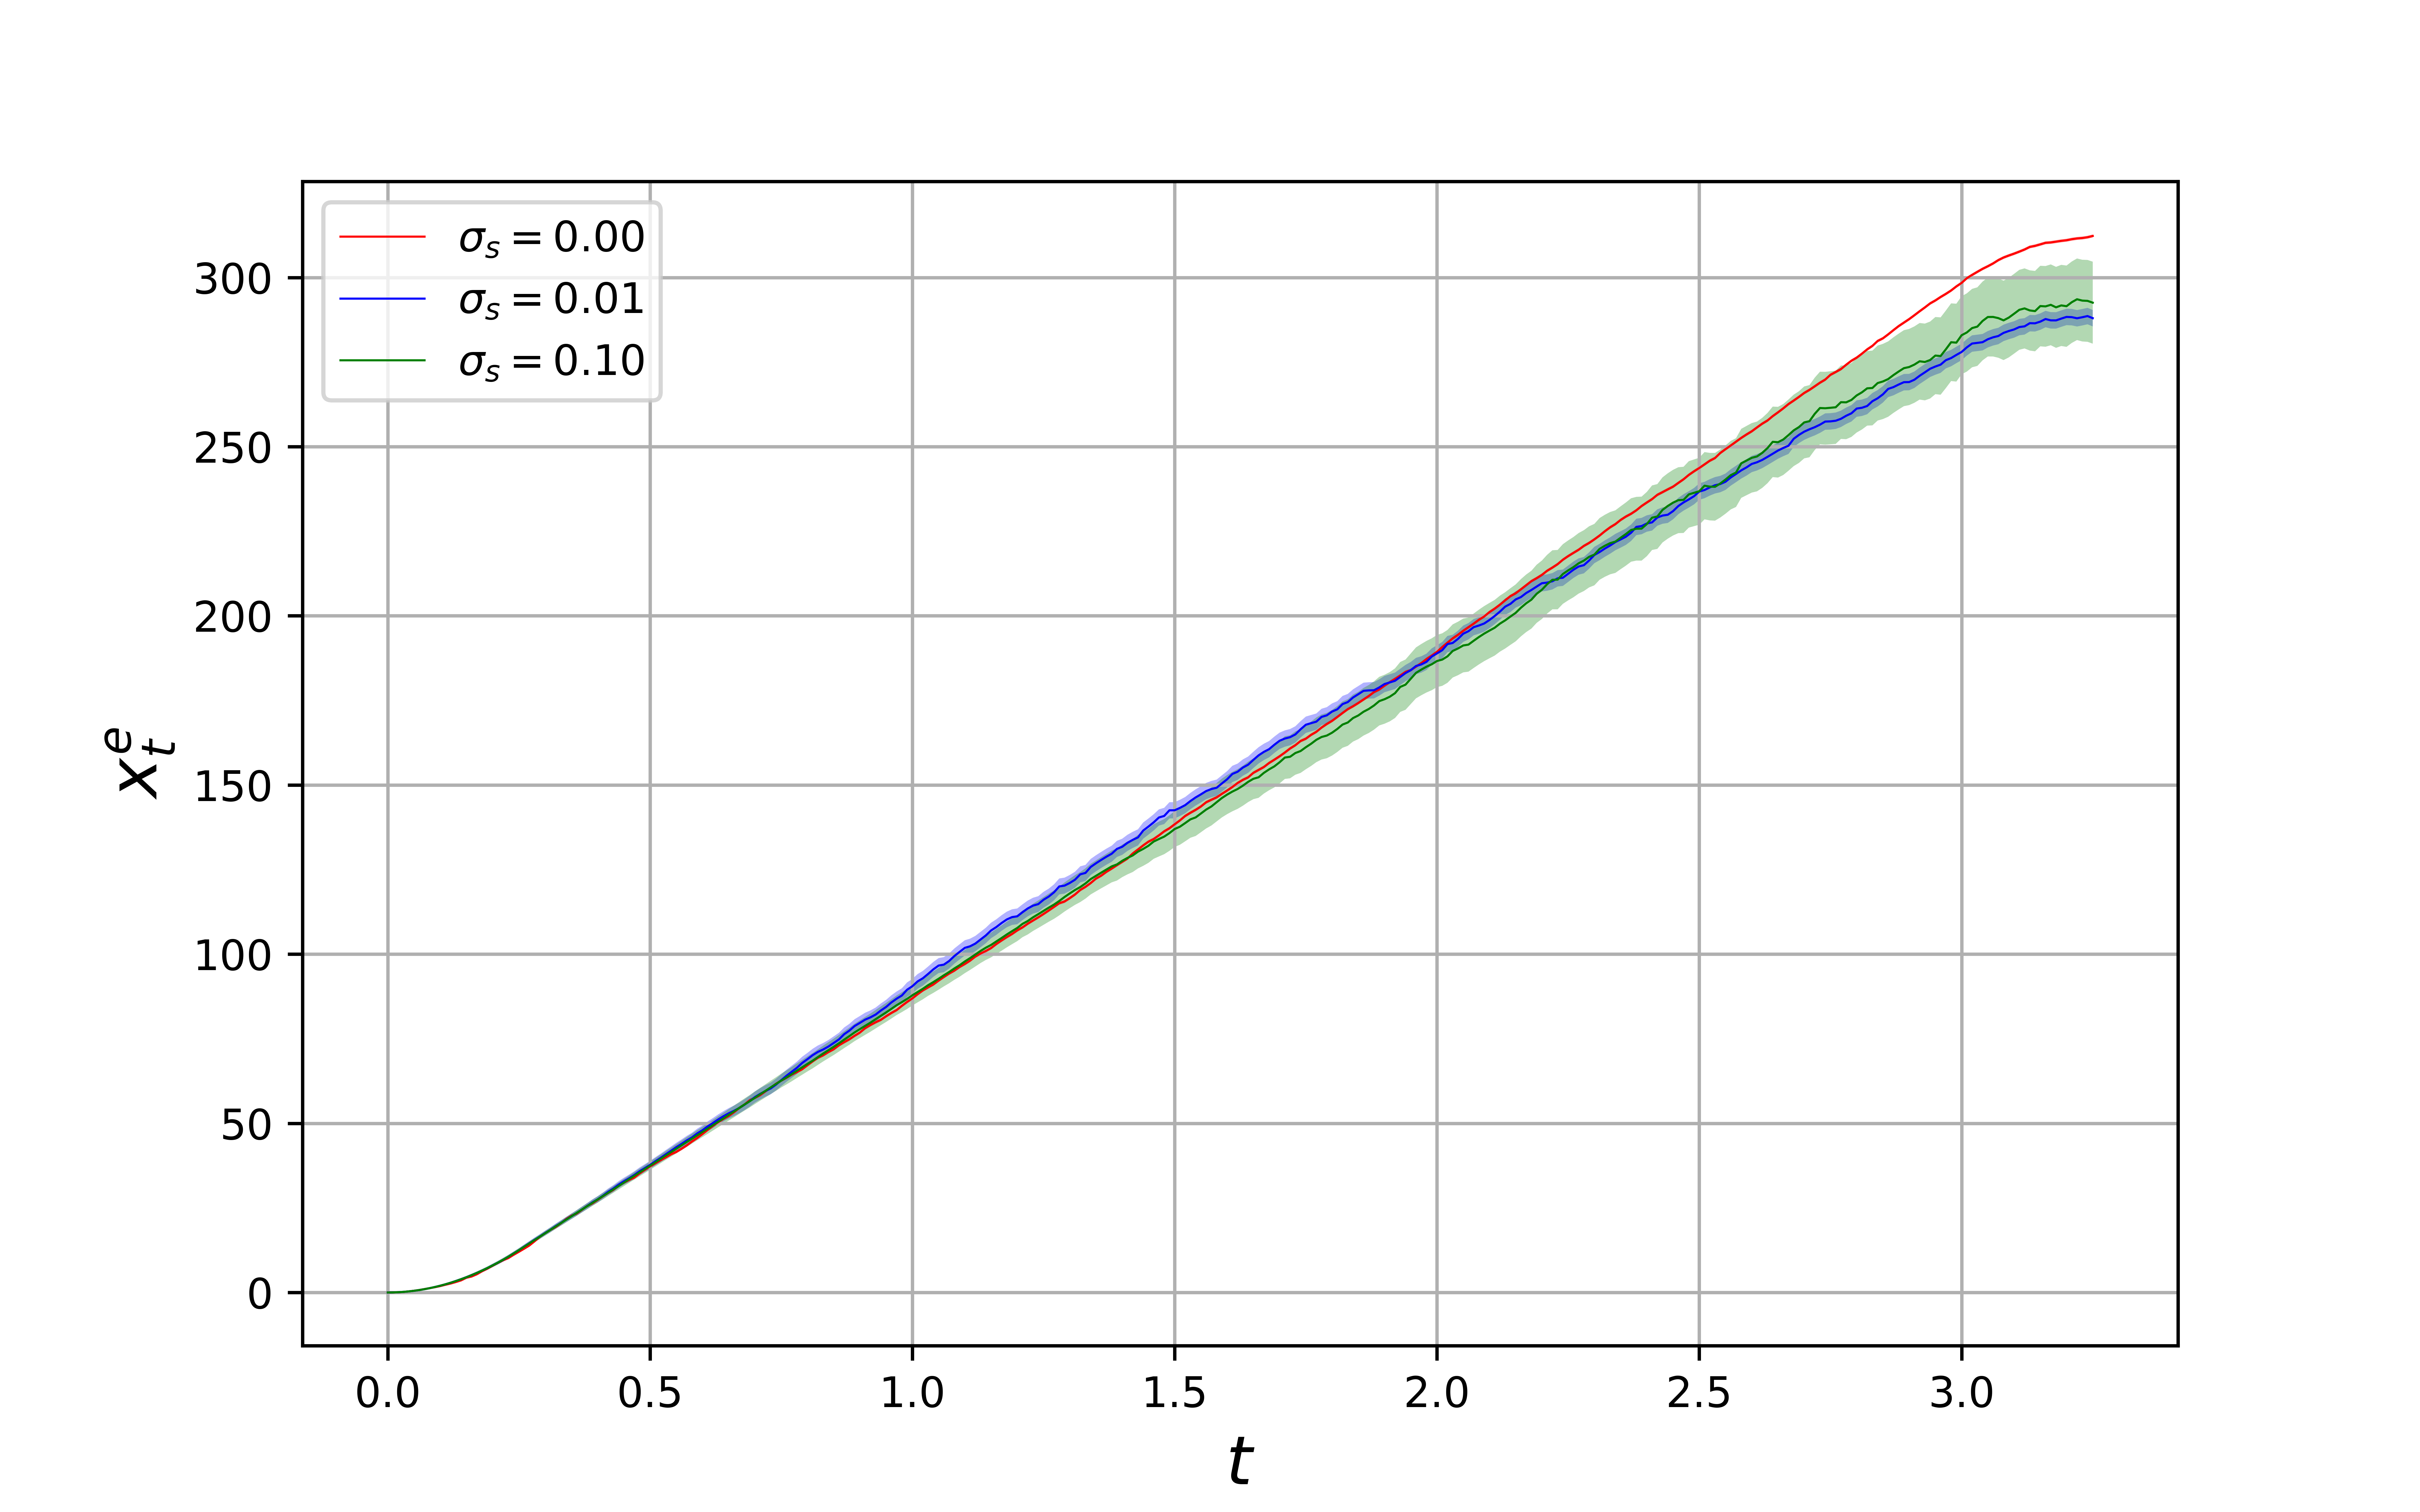
\includegraphics[width=\linewidth]{plots/part1-d.2-xe.png}
         \caption*{$x_t^e$ vs $t$}


    \end{minipage}
    \caption{Varying $\sigma_s = 0.001, 0.01, 0.1$}
    \label{fig:part1-vary-sigma_s}
    

\end{figure}

\subsection{Kalman Gain}
\begin{itemize}
\item 
A larger Kalman Gain implies that we trust the observations more, and update our belief (in the \textbf{Update Step}) more strongly as guided by observation, after the \textbf{Prediction Step}.

\item In \autoref{fig:part1-gain_sigma_s} we see that reducing $\sigma_s$ i.e. the expected error in sensor observations, increases both $K^{x}$ and $K^{\dot{x}}$.

\item In \autoref{fig:part1-gain_sigma_x} and \autoref{fig:part1-gain_sigma_x_dot} we see as $\sigma_x$ and $\sigma_{\dot{x}}$ are increased, the Kalman Gain increases. Intuitively, if the model expects the noise in the motion model to be larger, it trusts more on observations.

\item In all cases, as time passes, Kalman Gain increases, as the model starts trusting observations more, as the error in motion model keeps getting added.
 
\end{itemize}
\begin{figure}[H]
    \centering
    \begin{minipage}{0.49\linewidth}
        \centering
        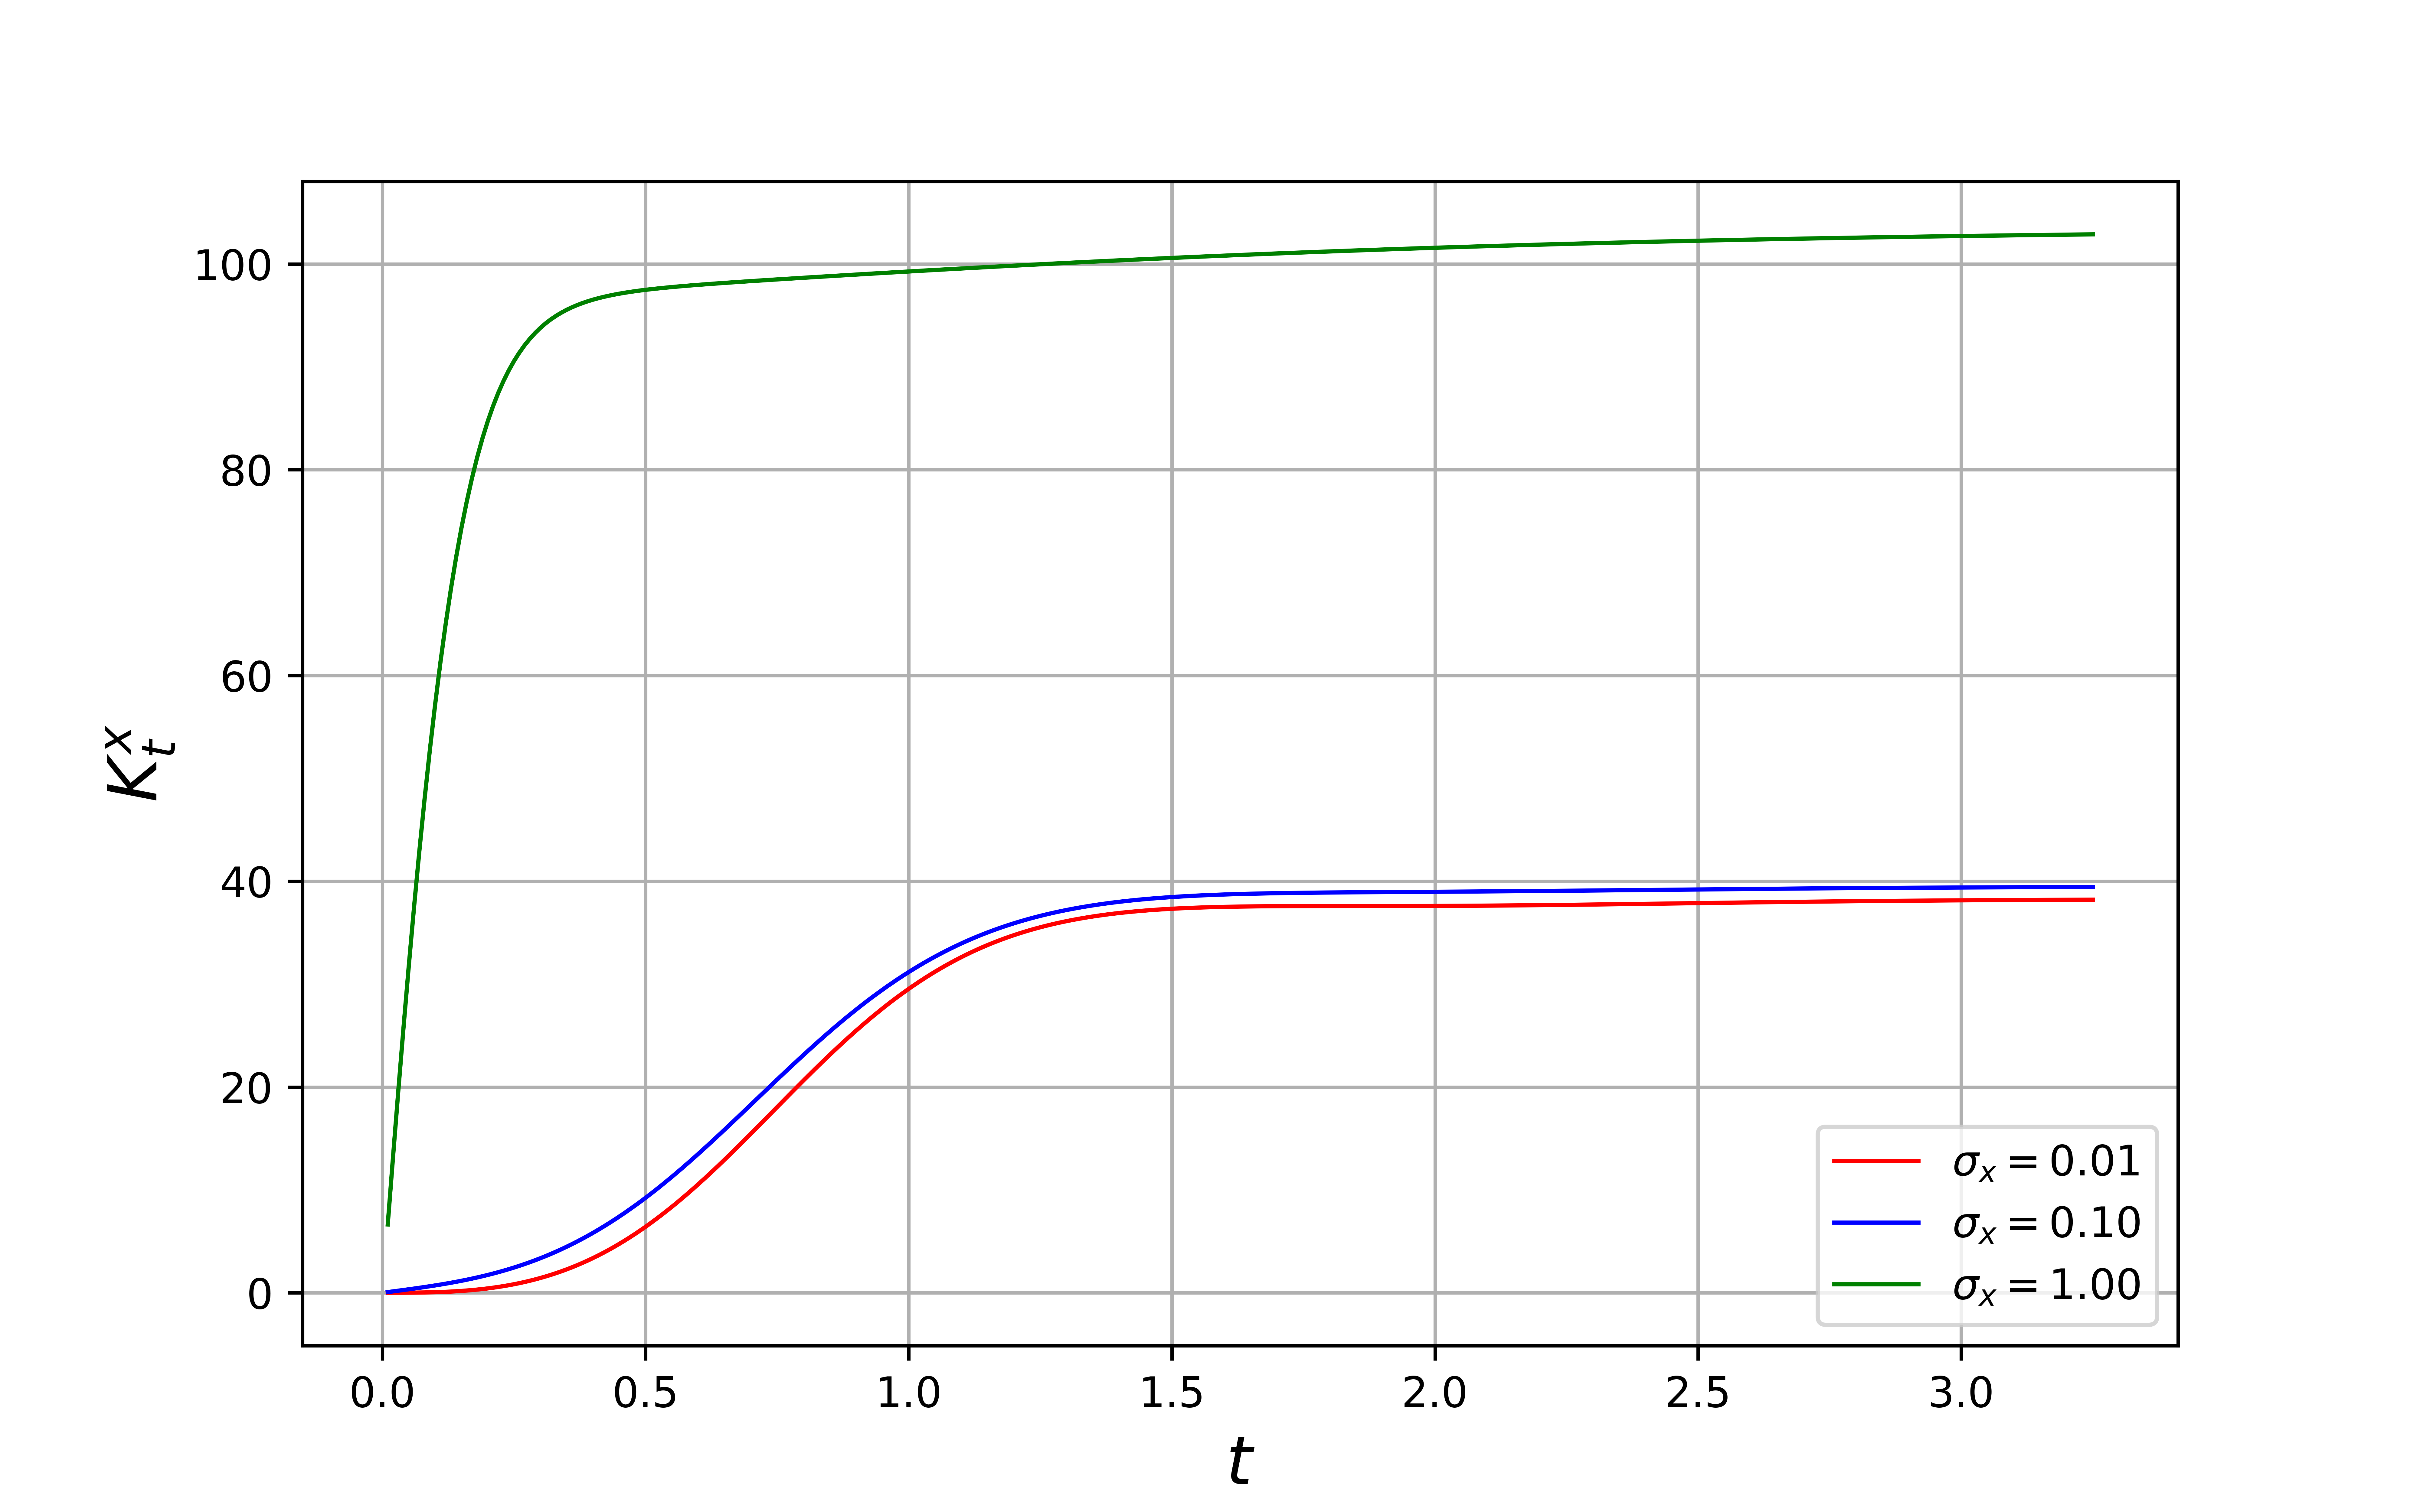
\includegraphics[width=\linewidth]{plots/part1-e.0-kx.png}
        \caption*{$K^x_t$ vs $t$}

    \end{minipage}
    \hfill
    \begin{minipage}{0.49\linewidth}
        \centering
        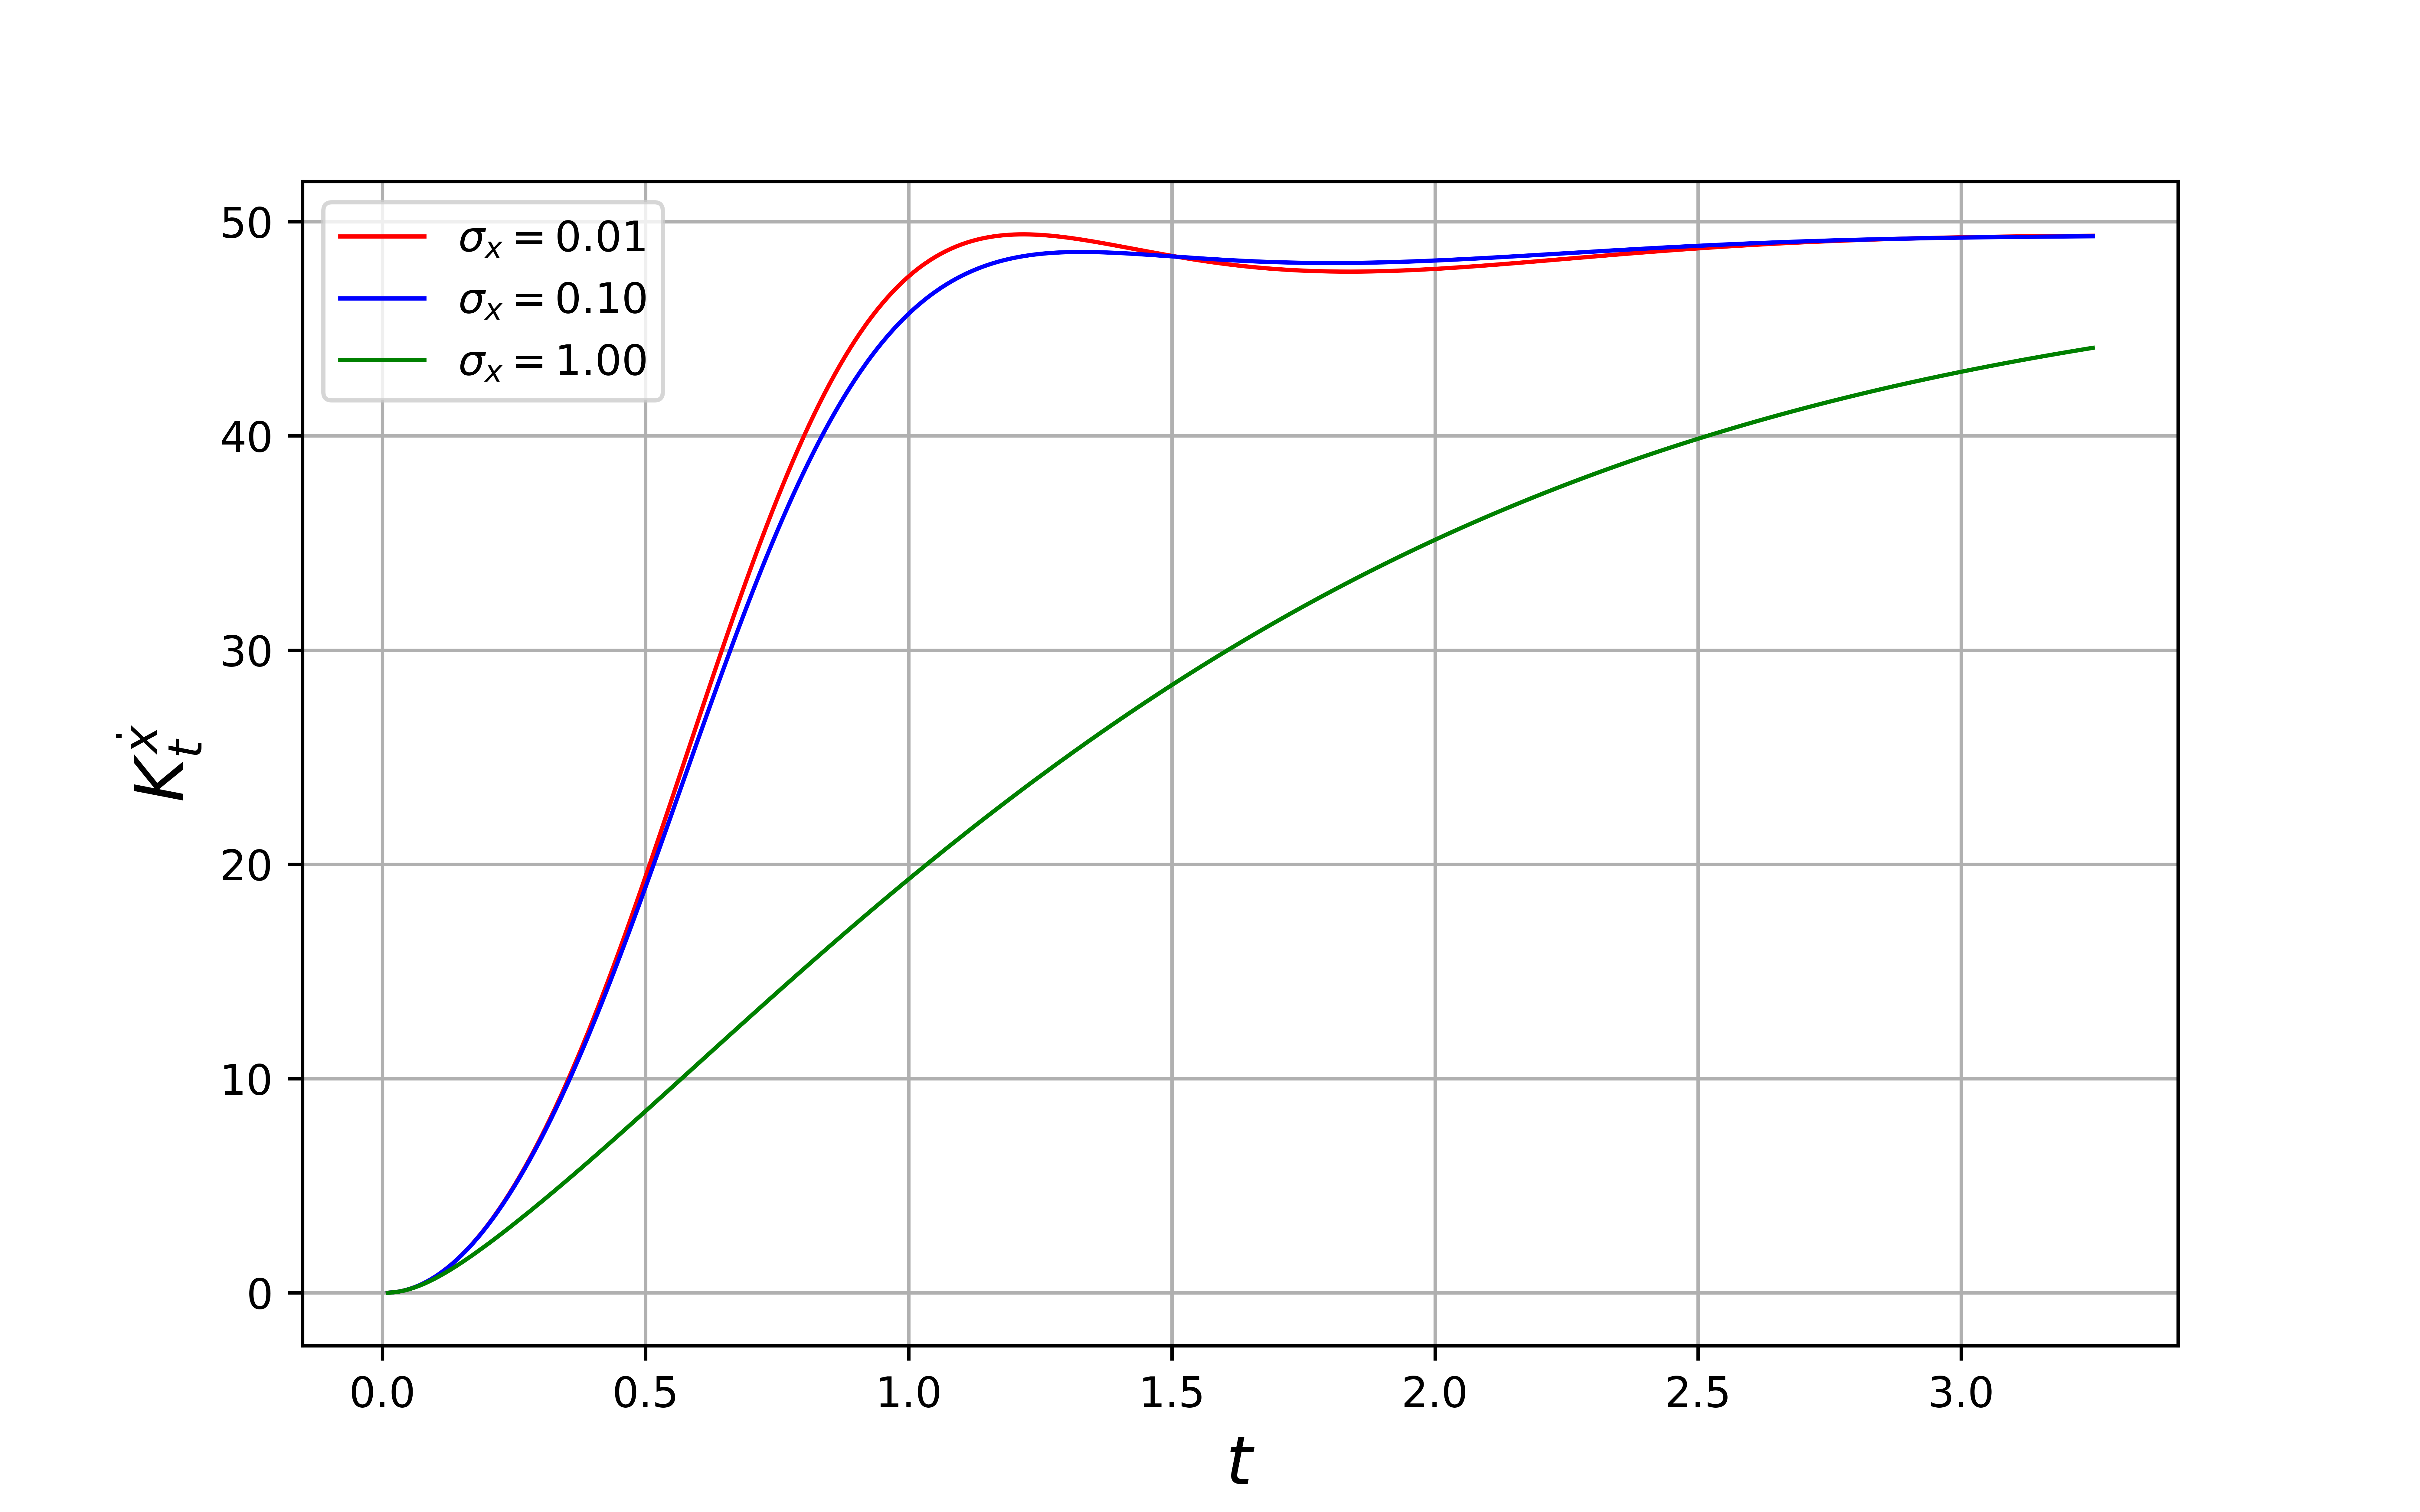
\includegraphics[width=\linewidth]{plots/part1-e.0-kv.png}
         \caption*{$K^{\dot{x}}_t$ vs $t$}
    \end{minipage}
    \caption{Varying $\sigma_x = 0.01, 0.1, 1.0$}
    \label{fig:part1-gain_sigma_x}
\end{figure}

\begin{figure}[H]
    \centering
    \begin{minipage}{0.49\linewidth}
        \centering
        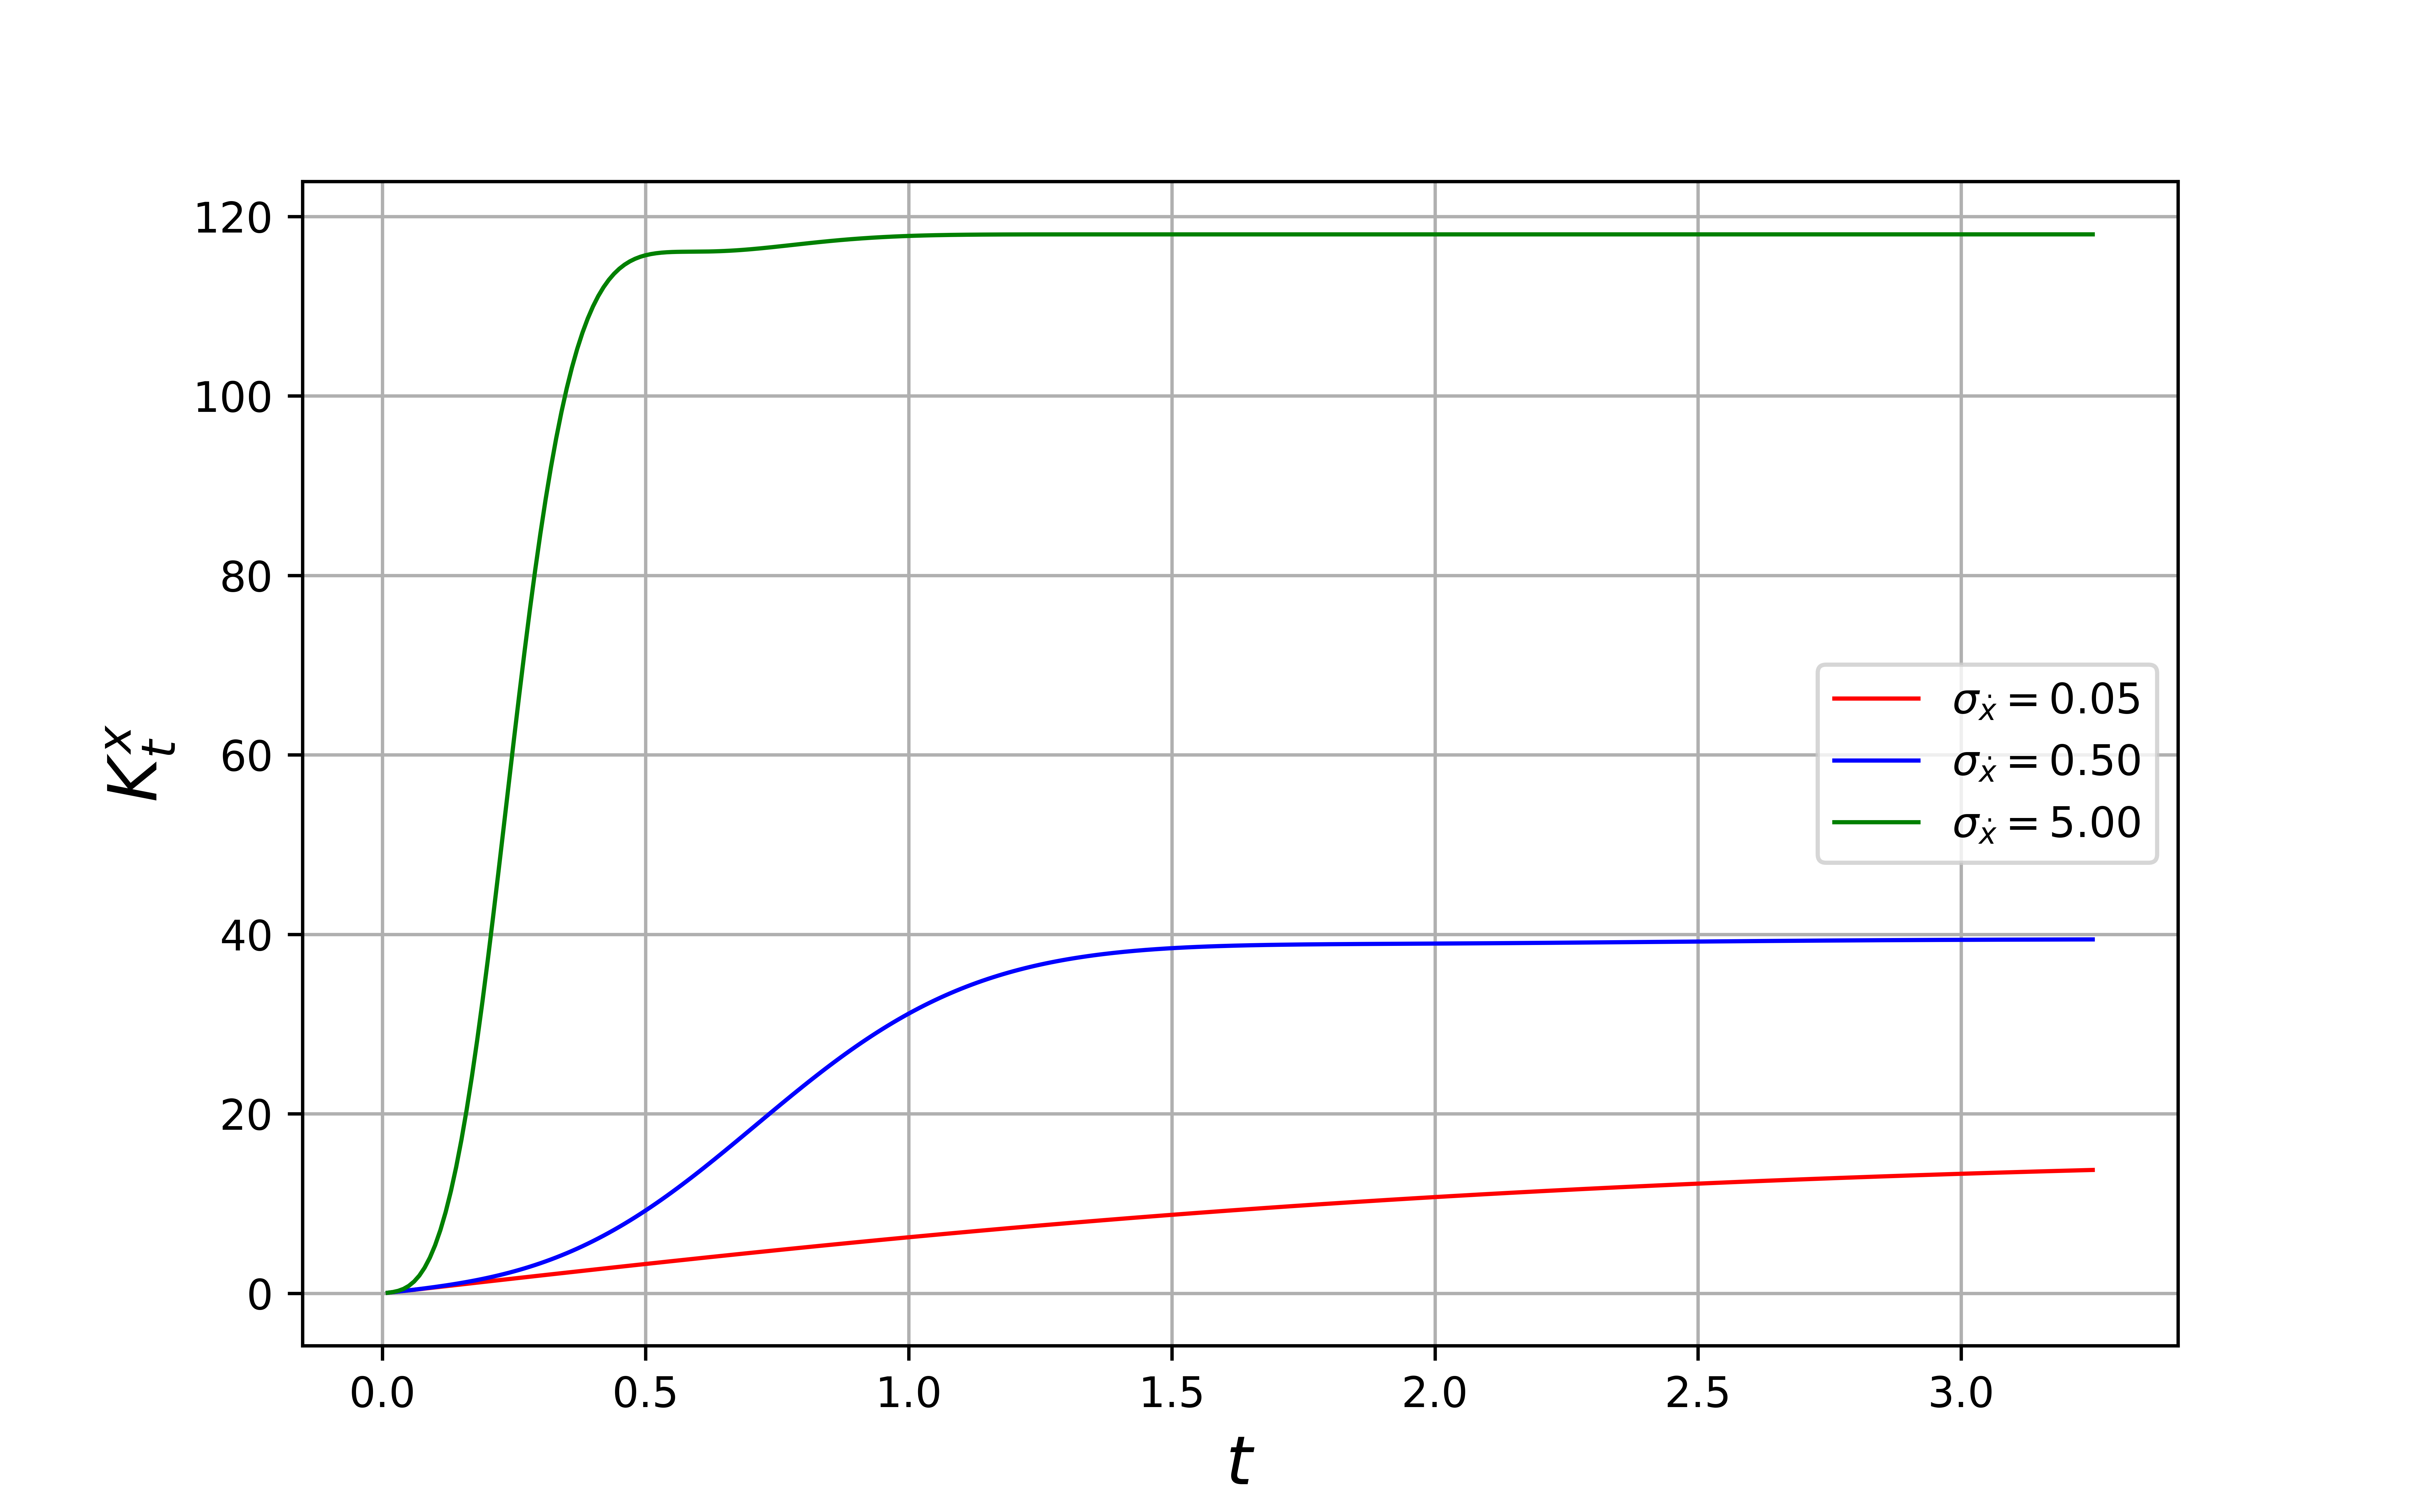
\includegraphics[width=\linewidth]{plots/part1-e.1-kx.png}
        \caption*{$K^x_t$ vs $t$}

    \end{minipage}
    \hfill
    \begin{minipage}{0.49\linewidth}
        \centering
        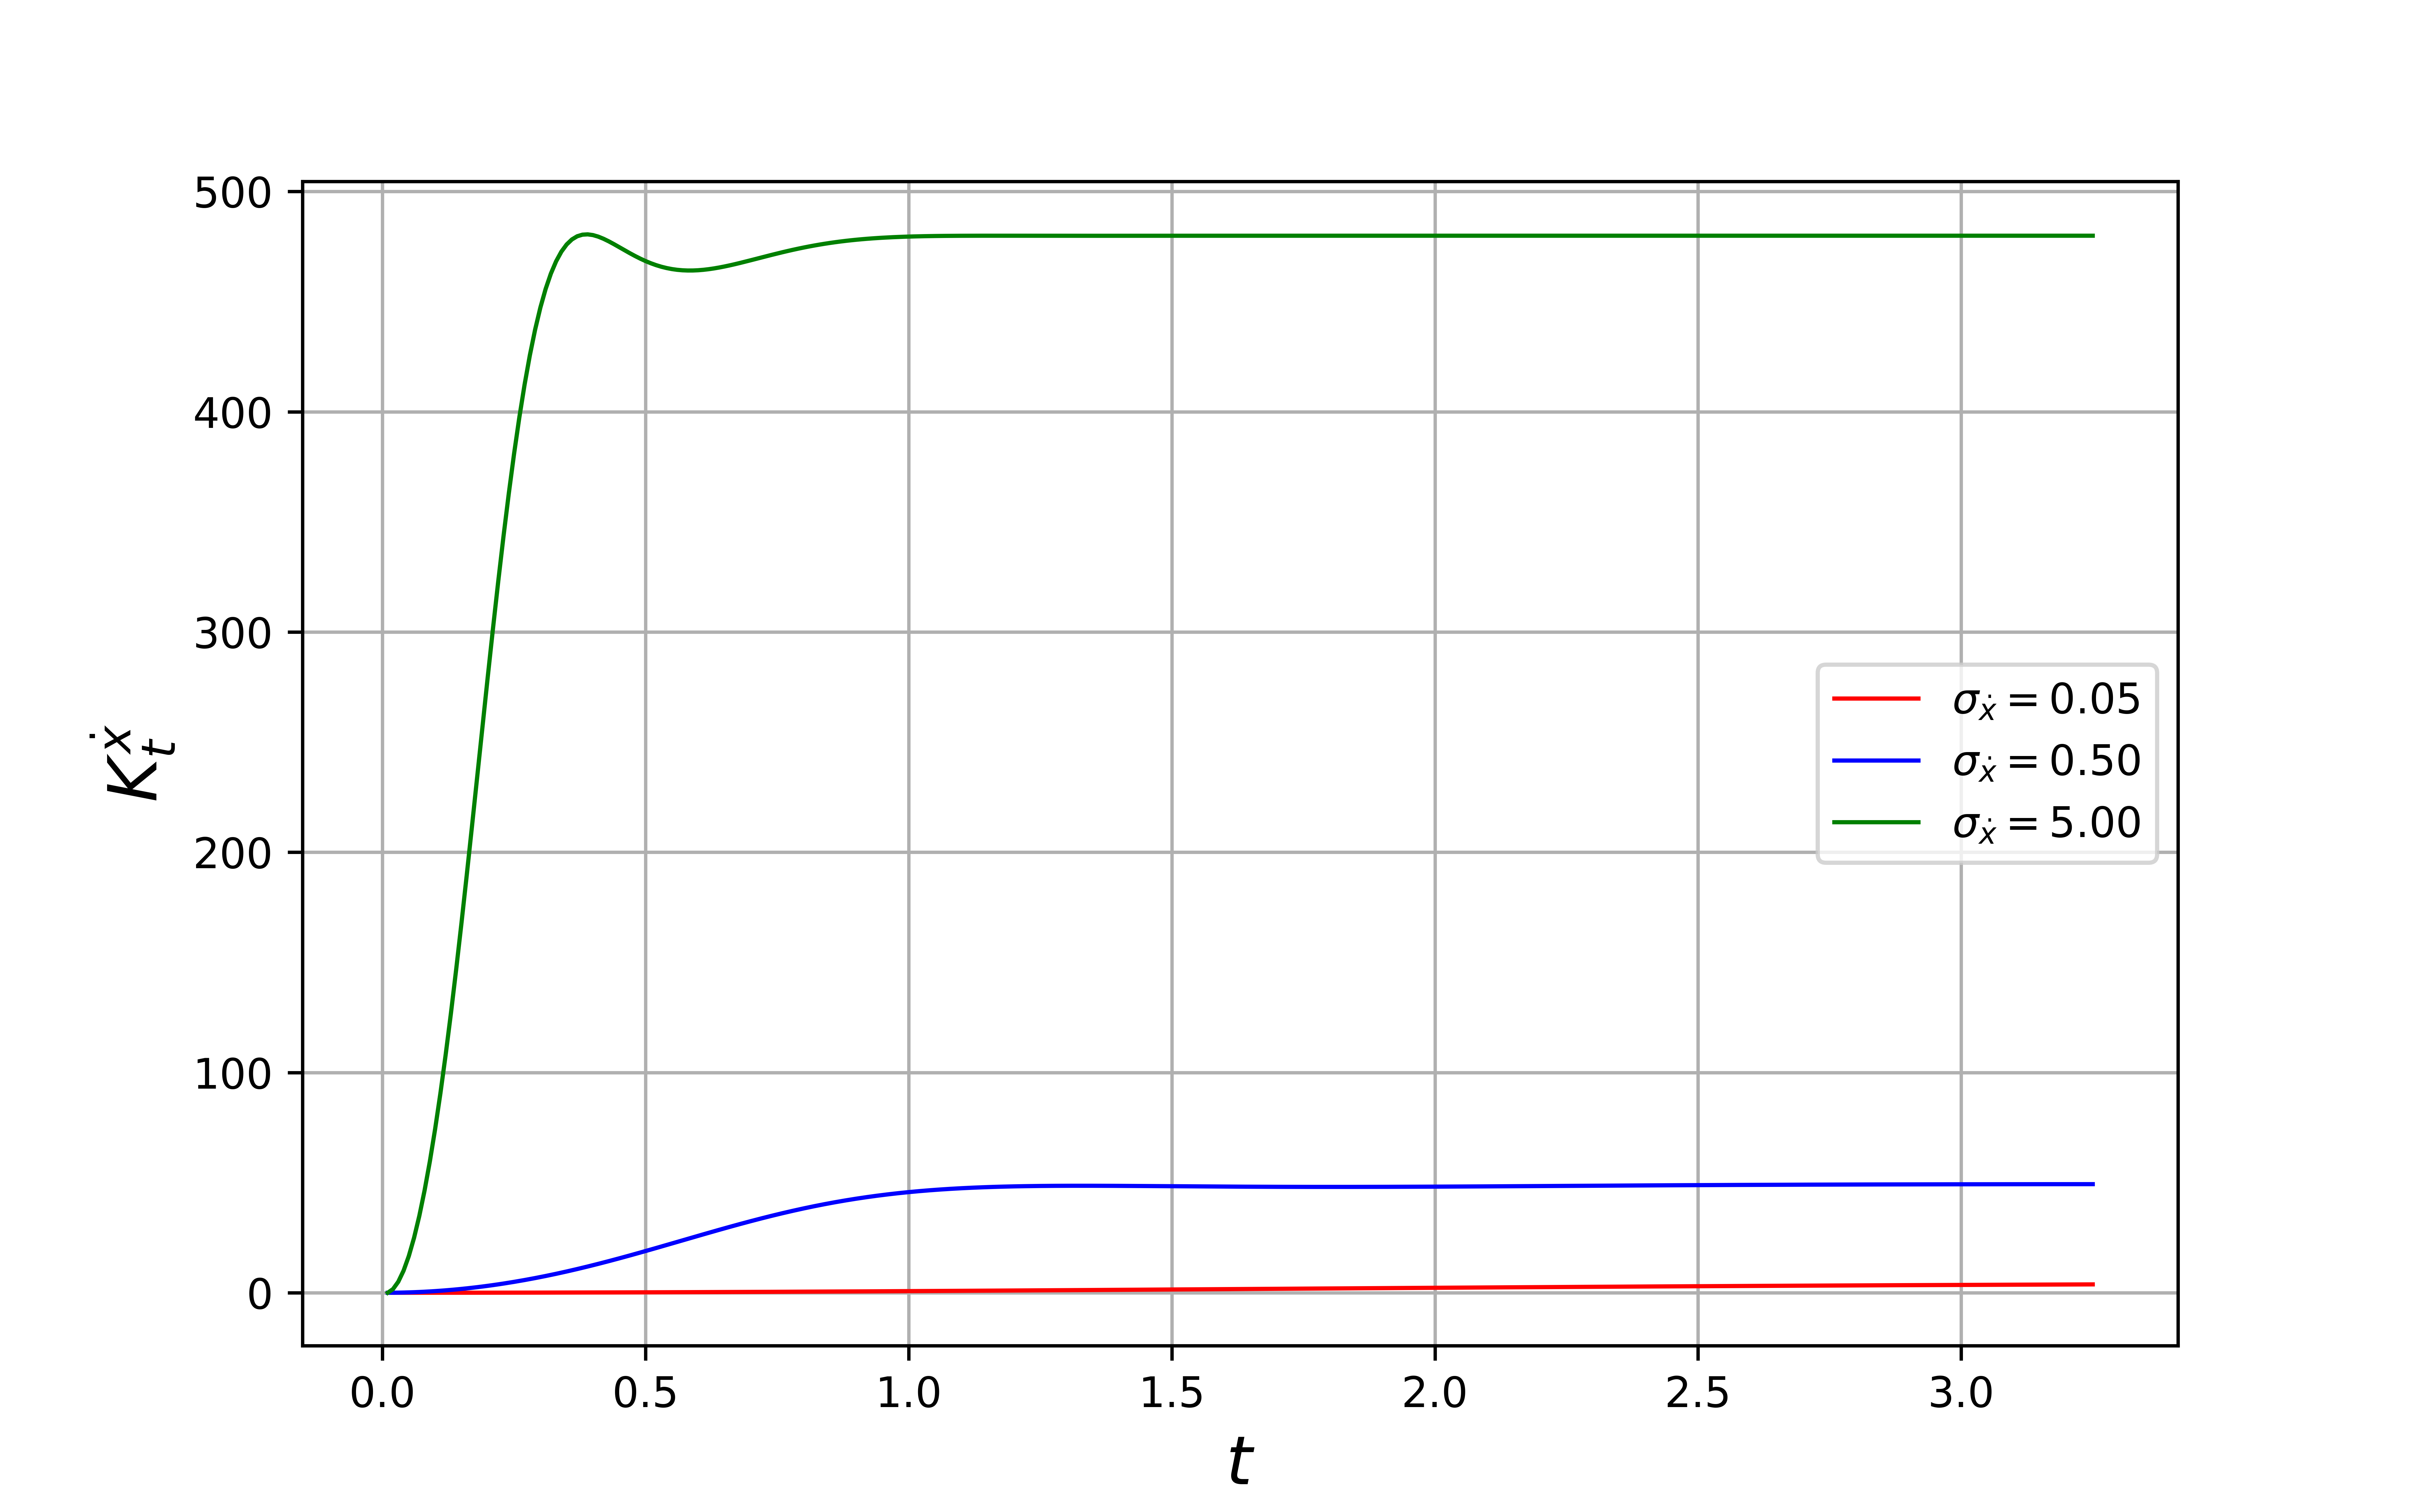
\includegraphics[width=\linewidth]{plots/part1-e.1-kv.png}
         \caption*{$K^{\dot{x}}_t$ vs $t$}
    \end{minipage}
    \caption{Varying $\sigma_{\dot{x}} = 0.05, 0.5, 5.0$}
    \label{fig:part1-gain_sigma_x_dot}
    
\end{figure}
\begin{figure}[H]
    \centering
    \begin{minipage}{0.491\linewidth}
        \centering
        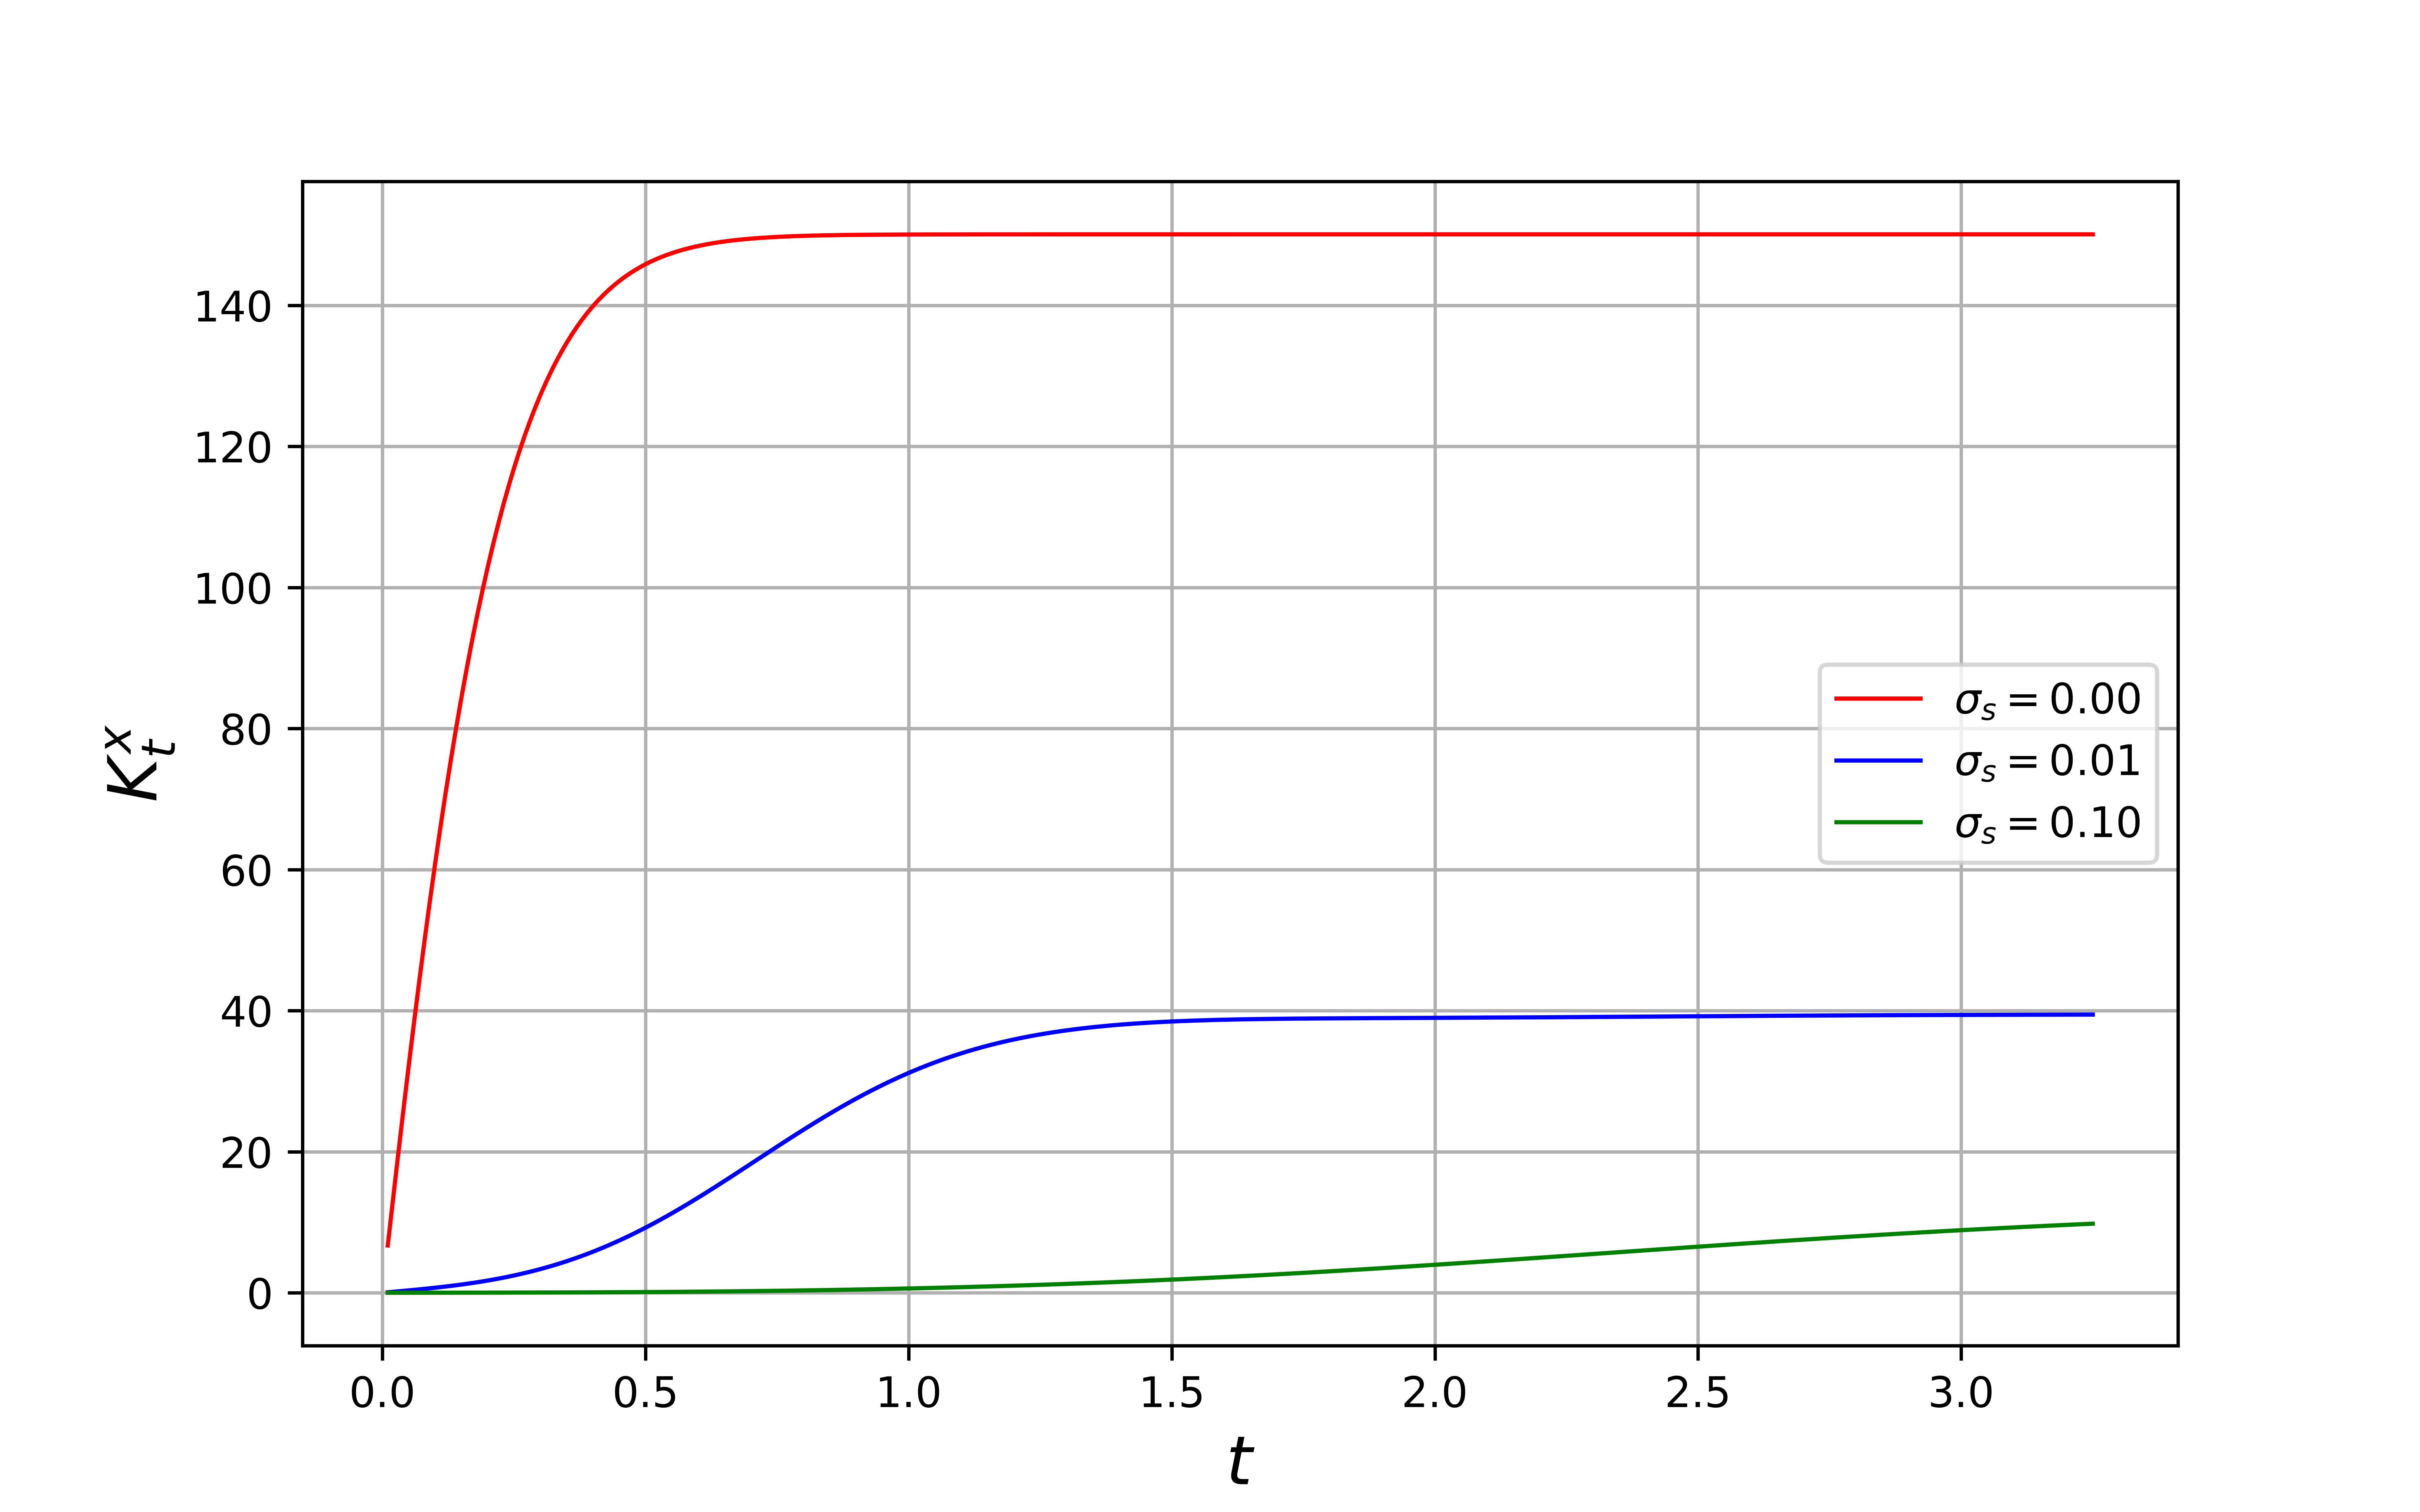
\includegraphics[width=\linewidth]{plots/part1-e.2-kx.png}
        \caption*{$K^x_t$ vs $t$}

    \end{minipage}
    \hfill
    \begin{minipage}{0.49\linewidth}
        \centering
        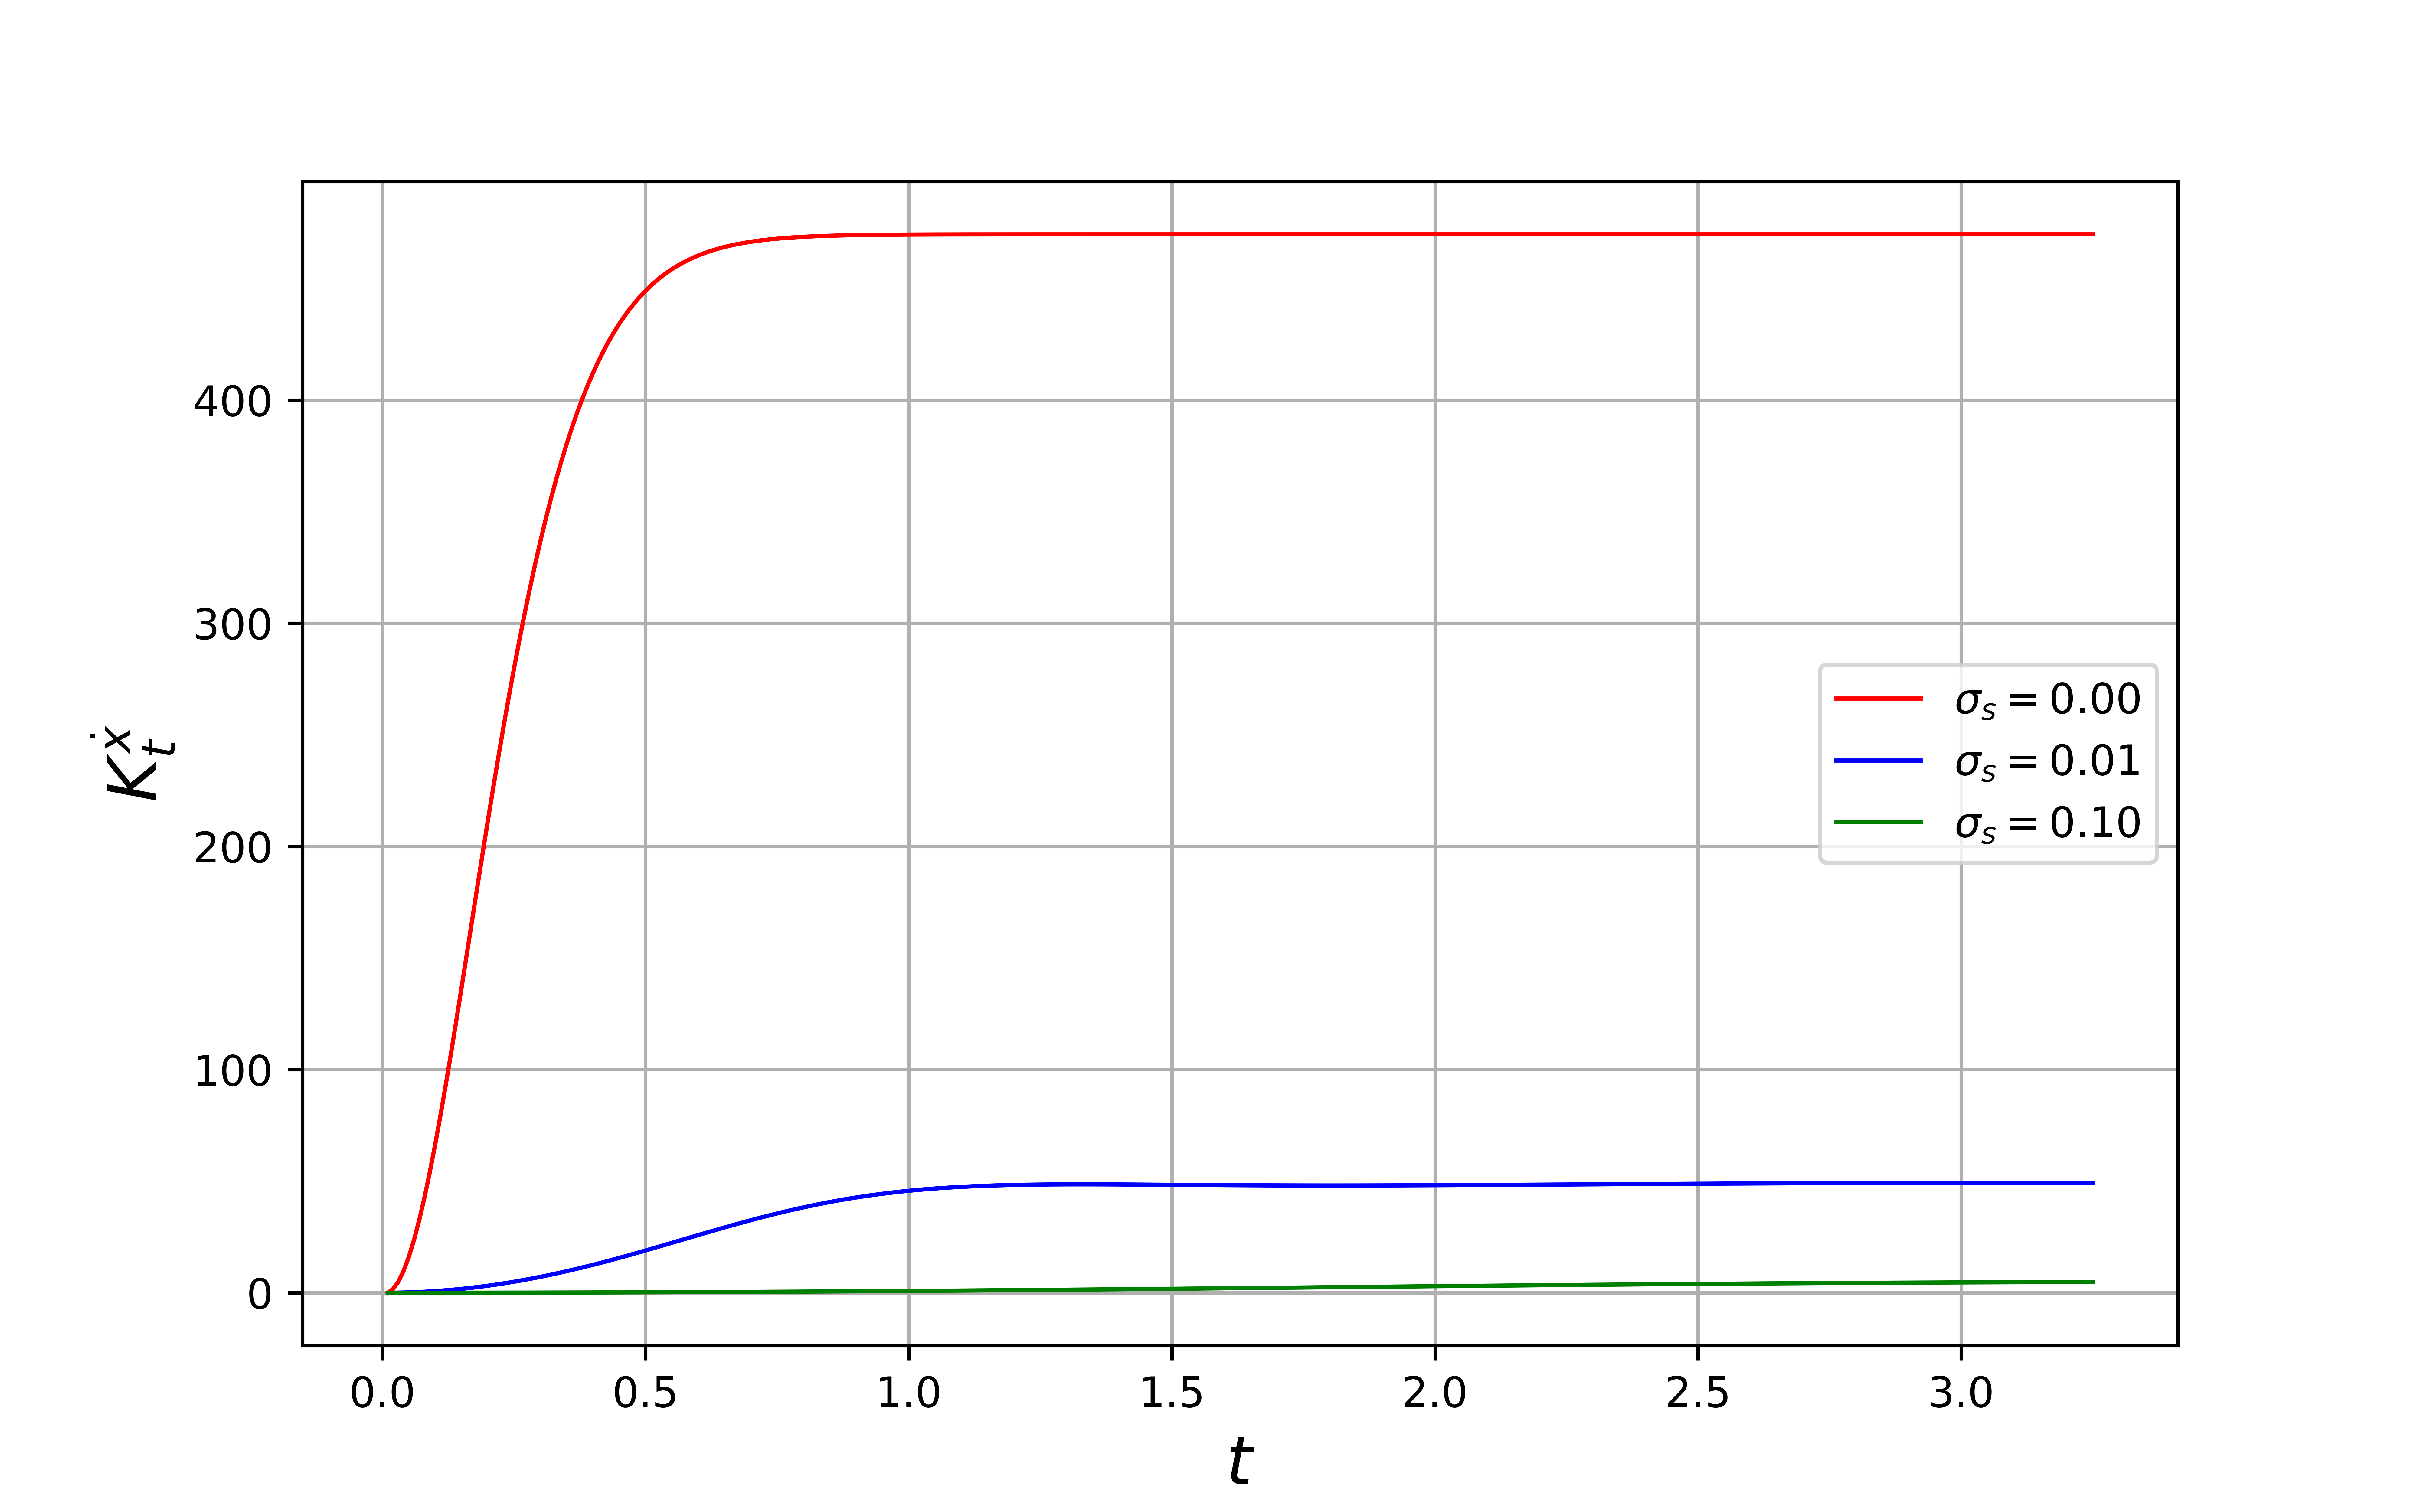
\includegraphics[width=\linewidth]{plots/part1-e.2-kv.png}
         \caption*{$K^{\dot{x}}_t$ vs $t$}
    \end{minipage}
    \caption{Varying $\sigma_s = 0.001, 0.01, 0.1$}
    \label{fig:part1-gain_sigma_s}
\end{figure}



\subsection{Missing Observations}
In \autoref{fig:missing-obs}, the width of uncertainty bar starts increasing more sharply after $t = 0.5$ (here observations are not available). After $t = 2.5$, the width starts reducing sharply, as observations are now available. The estimated trajectory still ends up very close to the ground truth, as the observations come back later.
\begin{figure}[H]
    \centering
    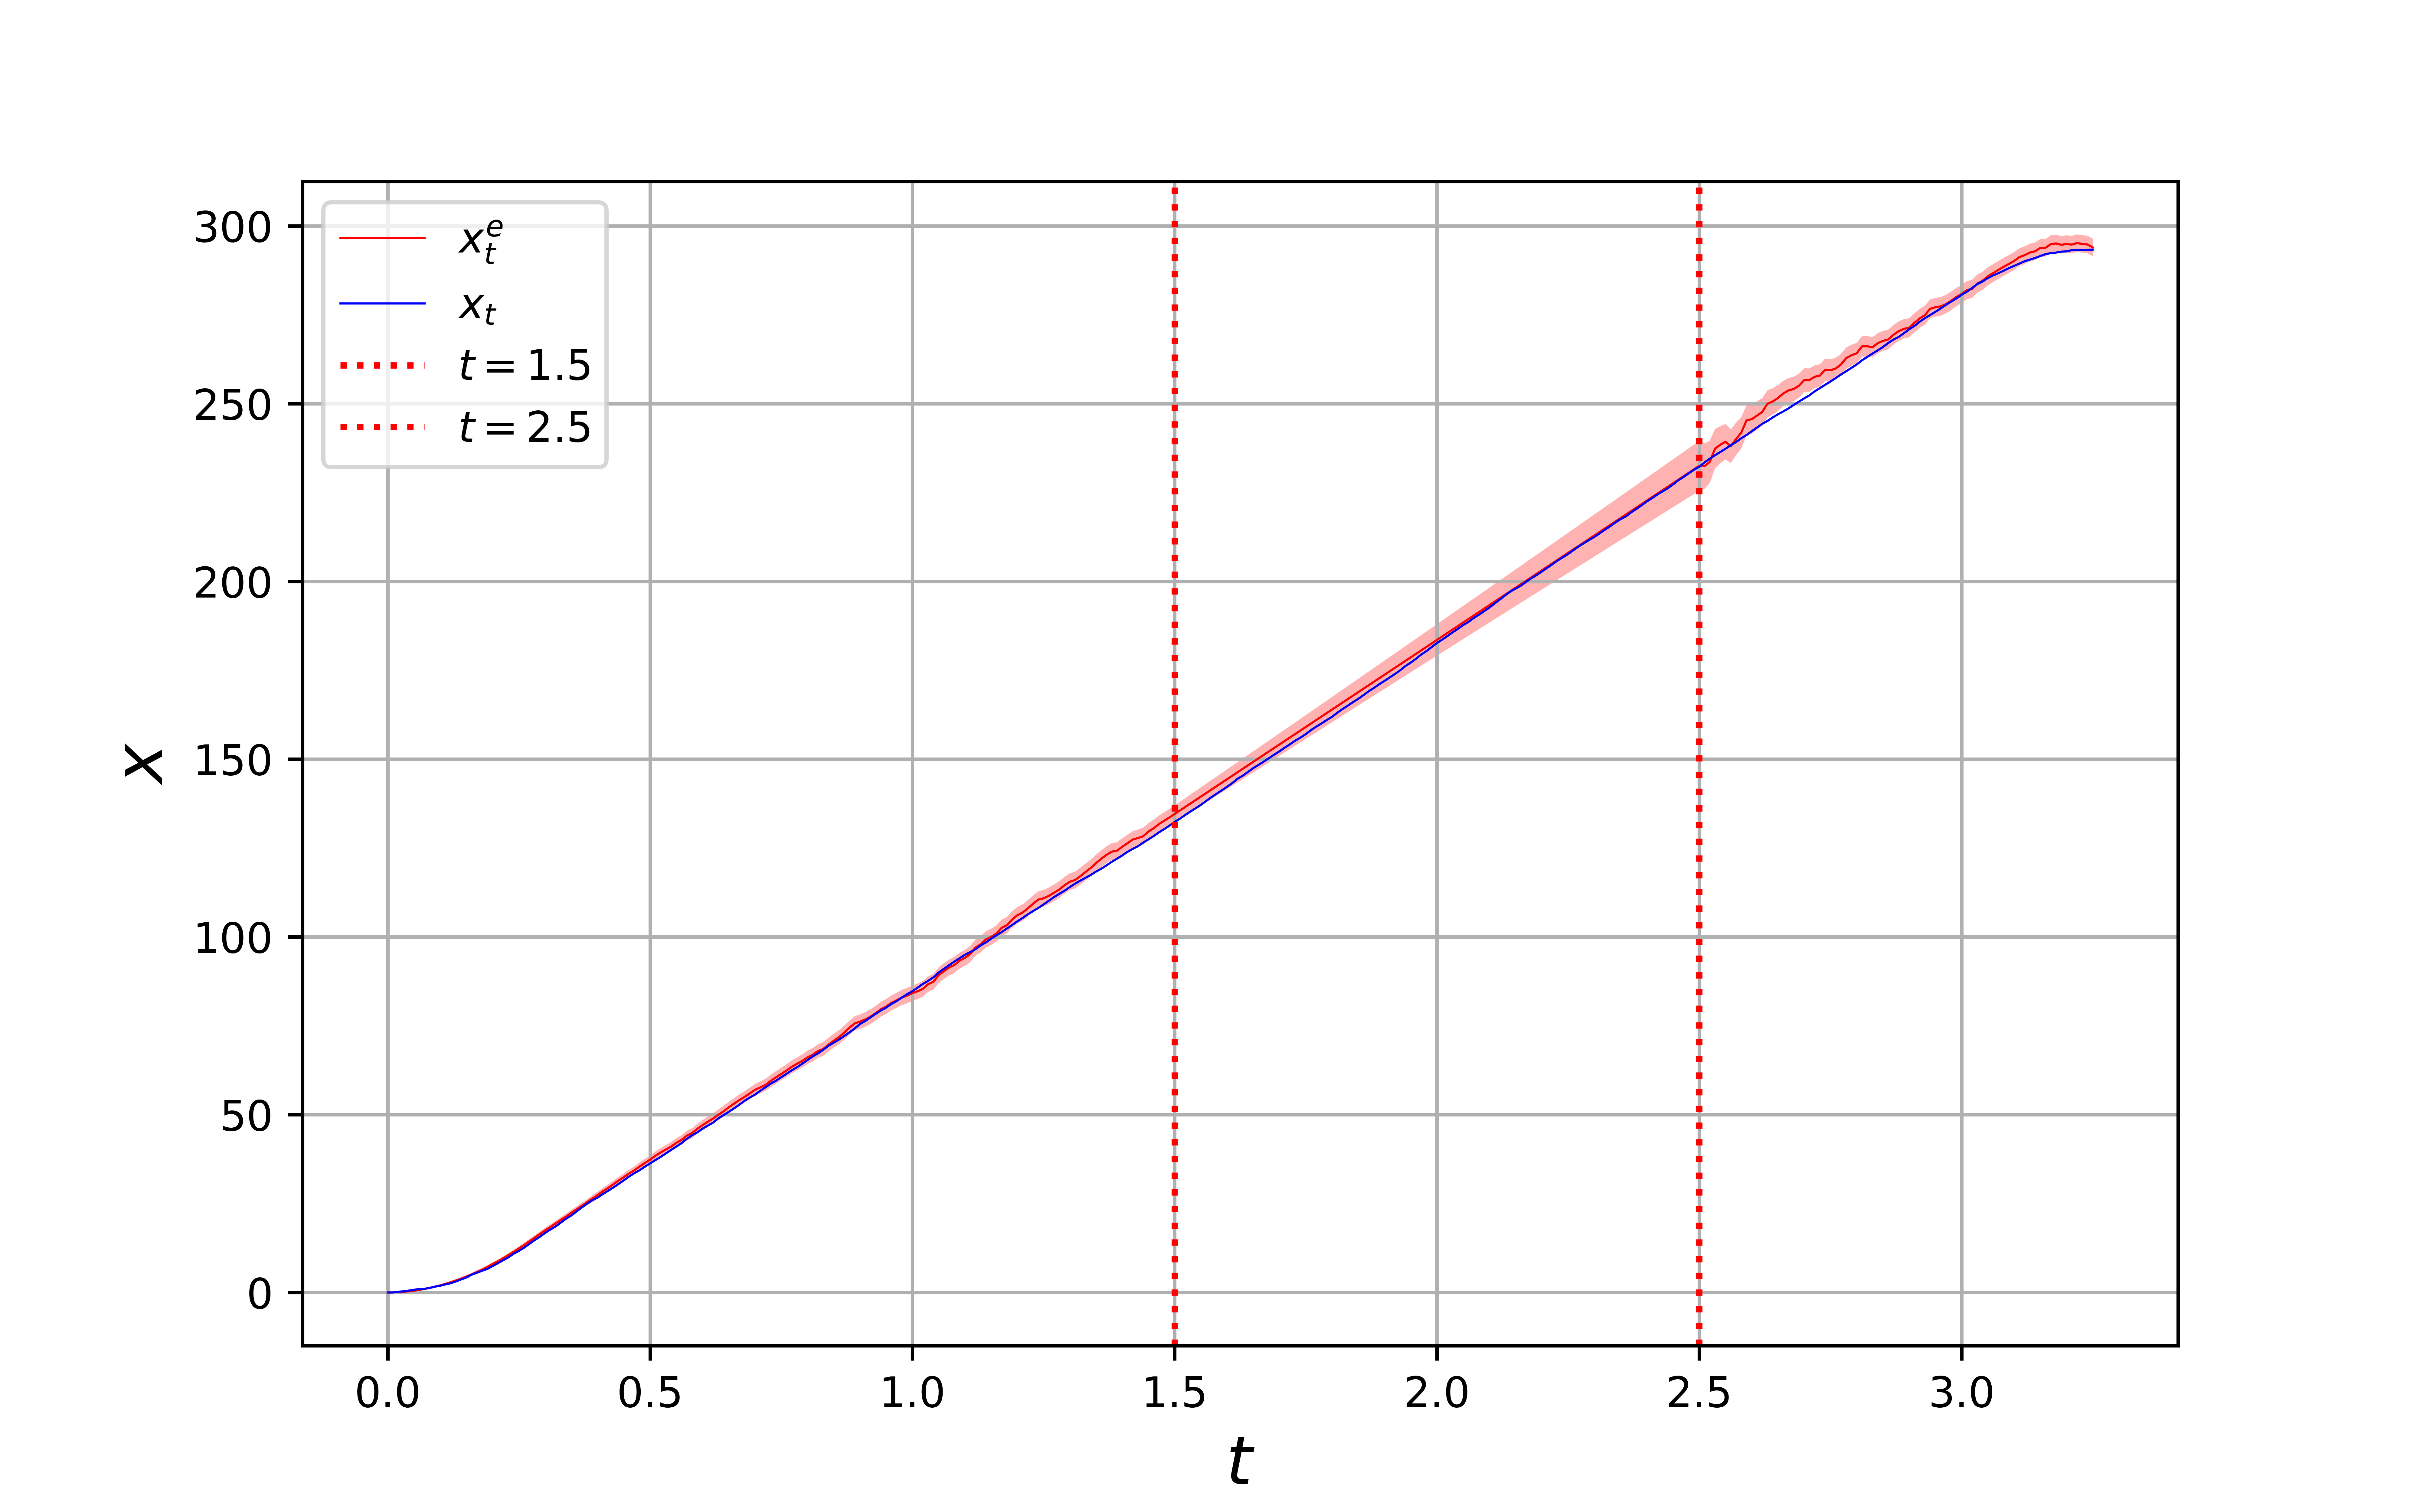
\includegraphics[width=1.0\linewidth]{plots/part1-f.png}
    \caption{Trajectory $x_t^e$ with missing observations in $t \in [1.5, 2.5]$}
    \label{fig:missing-obs}
\end{figure}
